\documentclass[10pt]{article} % For LaTeX2e
\usepackage{tmlr}
% Review PDF: \usepackage{tmlr}  (this file)
% Camera-ready: \usepackage[accepted]{tmlr} and restore CAMERA_READY_AUTHOR.txt
% Named preprint: \usepackage[preprint]{tmlr}

\usepackage{amsmath,amssymb}
\usepackage{xcolor}
\usepackage{booktabs,array,tabularx}
\usepackage{graphicx}
\usepackage{placeins}
\usepackage{hyperref}
\usepackage{url}
\usepackage{microtype}

\hypersetup{
  pdftitle={When Can Language Models Join Without Relation Names?},
  pdfauthor={Anonymous authors},
  pdfsubject={Unique-Path Traversal versus End-to-End Accuracy under Path Ambiguity},
  colorlinks=false,
  pdfborder={0 0 0},
  breaklinks=true
}
\graphicspath{{./}}
\emergencystretch=2em
\setlength{\textfloatsep}{8pt plus 2pt minus 4pt}
\setlength{\floatsep}{8pt plus 2pt minus 4pt}
\setlength{\intextsep}{8pt plus 2pt minus 4pt}
\setlength{\abovedisplayskip}{6pt plus 2pt minus 3pt}
\setlength{\belowdisplayskip}{6pt plus 2pt minus 3pt}
\setlength{\abovedisplayshortskip}{4pt plus 1pt minus 2pt}
\setlength{\belowdisplayshortskip}{4pt plus 1pt minus 2pt}

\title{When Can Language Models Join\\
Without Relation Names?\\
Unique-Path Traversal versus End-to-End Accuracy\\
under Path Ambiguity%
\thanks{Large language models were used as writing assistants for grammar
and phrasing. All ideas, claims, experimental design, locked numbers, and
scientific conclusions are the authors'.}}

% Hidden while tmlr is loaded without [accepted] or [preprint].
\author{\name Anonymous authors \email anonymous@openreview \\
 \addr Anonymous affiliation}

\def\month{09}
\def\year{2026}
\def\openreview{\url{https://openreview.net/forum?id=XXXX}}

\begin{document}
\maketitle

\begin{abstract}
We ask whether 2-hop answering over small labeled graphs needs readable
relation names, or only equality among identifiers.
Opaque isomorphic reasoning (OIR) replaces relation strings with keyed
opaque tokens, withholds a legend, and scores the answer node rather than
an emitted $(r_1,r_2)$.
A named-arm prompt names the condition in a one-line ARM header and uses
readable case ids; hashed-id packing keeps that ARM line and hashes the
ids; no-ARM packing drops the header.
Unique sealed routes---one 2-hop from a start already in the
question---still execute
(OpenAI unique English/opaque $200/200$;
hashed-id no-ARM $200/200$ at 512 tokens;
opaque unique $32/32$;
both-opaque unique $32/32$ on three families).
When two complete same-type 2-hops compete and no hop is written, a
CONTEXT-only instruction makes \texttt{UNKNOWN} the appropriate reply:
CONTEXT gives no explicit cue for one city.
Named-arm OpenAI usually yields that reply, not the decoy: $38/200$ gold,
\texttt{UNKNOWN} $151$, decoy $11$.
English two-path is $199/200$ under the same instruction, so the format
does not force abstention when names identify a route.
Packaging reduces abstention on those same two-path graphs, not a
packaging-free opacity law
(\texttt{UNKNOWN} $151\to 44$ with hashed case ids, ARM line kept,
gold $134/200$, decoy $20$;
\texttt{UNKNOWN} $5$ with the header dropped at 4096/medium).
Dropping the header, at 4096 tokens and reasoning effort medium, is a
two-path cell (unique-path was not run at that budget):
cyclic-decoy English two-path is $197/200$ and opaque two-path is
$174/200$.
Entity names stay English and we score the answer node, not $(r_1,r_2)$,
so two-path exact-match cannot be attributed to a join over CONTEXT.
English relation names restore OpenAI with anonymous entities
(opaque-entity two-path $32/32$ vs.\ both-opaque $1/32$).
HMAC-SHA256 is one generator of that renaming on each instance's finite
atom set, not a cryptographic or privacy primitive.
On the primary $2{\times}2$, seals hide relation strings; entity names
remain. They are not a confidentiality proof.
\end{abstract}

\section{Introduction}

The scored Wikidata question is \emph{What city is the headquarters of the
company led by \mbox{Michael Eisner}?}
English unique-path context walks \texttt{works\_at} then
\texttt{headquartered\_in} to Burbank. That success may use English
predicates, or only equality among identifiers.
The two-path decoy is an injected second person$\to$company$\to$city route
(\texttt{partner\_of}/\texttt{located\_in}) to Kansas City, not a Wikidata
fact.
Opaque two-path keeps the English question and entity names; those
predicates become keyed opaque tokens (\texttt{works\_at} $\mapsto$
\texttt{E334675310f05} on the scored Eisner item).

\textbf{Opaque isomorphic reasoning (OIR)} measures whether a model can
join after English predicate strings are replaced by keyed opaque tokens,
with no legend in the prompt.
HMAC-SHA256 is the generator used here.
A 2-hop factors as two inferred maps; we score only the answer node:
selection $q \mapsto (r_1,r_2)$ and traversal
$(v_0,r_1,r_2,G)\mapsto v_2$.
Opacity does not, by itself, block traversal.
The question is when the prompt no longer maps query semantics onto one of
two sealed relation sequences.
Putting the start entity in $q$ as the same atom as in $V$
(\textbf{start in $q$}) separates that question from start-entity
identification.
On the primary $2{\times}2$, ``lexical cues'' means relation strings
(entities stay English); both-opaque is a separate ablation.
That suite is \textsc{Wiki-H5}.
Prompts differ in how they name the condition: a readable header and case
id (named-arm), the same header with hashed ids, or no header
(Section~\ref{sec:method}).

This paper reports three measurements.
(i)~Unique sealed routes still execute with the start in $q$ and no written hop.
(ii)~Under two competing sealed routes, OpenAI on
\texttt{OPAQUE\_AMBIG} usually answers
\texttt{UNKNOWN}, not the decoy.
Under a CONTEXT-only instruction that is the appropriate reply: two
same-type 2-hops are in CONTEXT and no hop is written, so CONTEXT gives no
explicit cue for one city (Section~\ref{sec:method}).
(iii)~Matched demonstrations restore shown seals; novel seals are a
negative control whose expected gold is near zero.
Packaging moves the abstention rate on the same two-path graphs
(Figure~\ref{fig:spine}; Section~\ref{sec:header}).
That packing result, including a two-path no-ARM English/opaque pair at
4096/medium, is not an opacity$\times$topology law: unique-path was not
run at that budget.
What is new is abstention on the \texttt{OPAQUE\_AMBIG} prompt
(condition label in the id and H5 header) when opacity meets path ambiguity
(Section~\ref{sec:fact2x2}), and how large a prompt-surface move can be
on the same sealed graph (Section~\ref{sec:header}).

\begin{figure}[t]
\centering
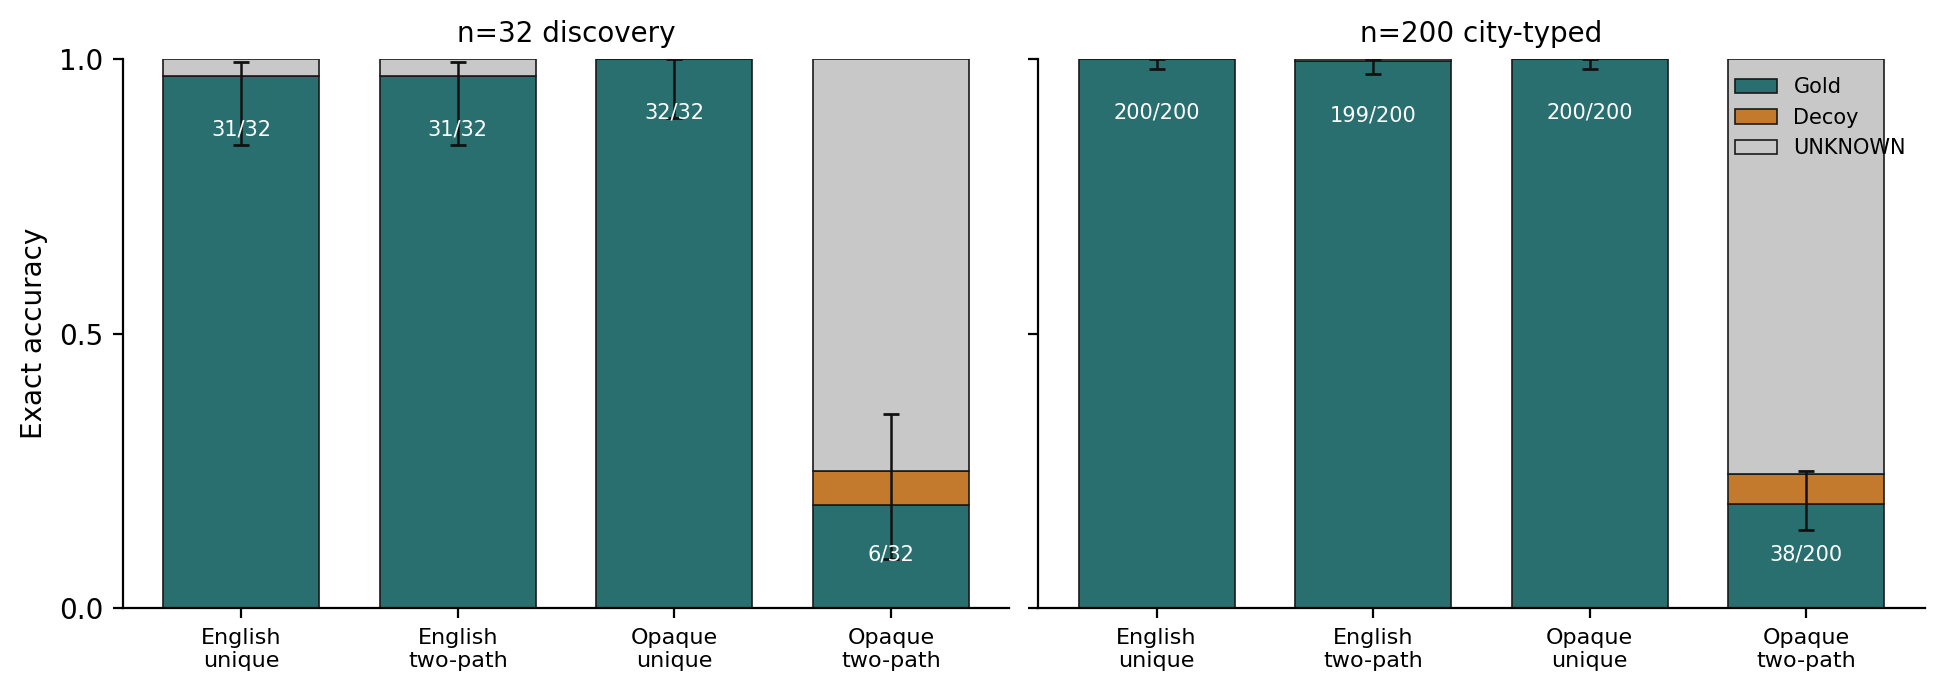
\includegraphics[width=0.92\linewidth]{fig1_matched_2x2.png}
\caption{OpenAI \textsc{Wiki-H5} (start in $q$).
Stacked bars are gold / decoy / \texttt{UNKNOWN}; whiskers are Wilson 95\%
intervals.
The usual named-arm reply is \texttt{UNKNOWN}, not the decoy.
Left: $n{=}32$ named-arm lock (August; opaque two-path \texttt{UNKNOWN} $24$,
decoy $2$, gold $6/32$).
Middle: city-typed $n{=}200$ named-arm (\texttt{UNKNOWN} $151$, decoy $11$,
gold $38/200$).
Right: same $n{=}200$ graphs and ARM line, hashed case ids (packing on the
same two-path graphs, not the named-arm headline)
(gold $134/200$, \texttt{UNKNOWN} $44$, decoy $20$;
remainder other $1$, \texttt{NO\_OUTPUT} $1$).
No-ARM two-path at 4096/medium is Table~\ref{tab:headerdecoy200}.
Alias $k{=}3$ is Table~\ref{tab:modes}.}
\label{fig:spine}
\end{figure}

\section{Related Work}

Think-on-Graph and Reasoning-on-Graphs select the next readable
relation~\citep{sun2024tog,luo2024rog}. Ciphered ICL is not path ambiguity on a
labeled graph~\citep{fang2025ciphers,guo2025ciphered}.
GSM-Symbolic swaps entity names in English math and templates some
numerical values~\citep{mirzadeh2025gsm};
2WikiMultihopQA is a readable multi-hop control~\citep{ho2020constructing}.

ARoG anonymizes \emph{entities} while relations stay the retrieval
language~\citep{arog2025}. PrivGemo HMAC-seals entities ($\phi_Q$, e.g.\
\texttt{ent\_17}); relations stay original labels or clustered schema words,
not keyed opaque tokens, and a local Hand answers on the raw graph after a
remote Brain ranks retrieved paths (CWQ $67\%$ plaintext $\to$ $59\%$ fully
anonymized; WebQSP $75\%$ fully anonymized)~\citep{privgemo2026,talmor2018cwq,yih2016webqsp}.
CoR explores readable relations because entities often have no semantics
beyond opaque IDs --- CoR's opaque-entity hide-set, not relation-only
\textsc{Wiki-H5}~\citep{liu2026cor}.
\citet{tang2023semantic} find LLMs fail when relation names are replaced by
symbols (\texttt{r1}) and rules must carry deduction; OpenAI unique-path
opaque $32/32$ is the complementary case: sealed relations still traverse
when topology fixes the route.
\citet[section 2.2]{guo2025twohop} report collapse to random guessing among end entities
when distractor two-hops have other sources. Named-arm Wiki-H5 opaque
two-path, with \texttt{UNKNOWN} allowed, is abstention rather than guessing
(Section~\ref{sec:fact2x2}, Table~\ref{tab:modes}).
A forced-choice arm is not in this evaluation
(Section~\ref{sec:limitations}) and would put those protocols on the same
scale.
OIR withholds a retrieved-path ranking and a local plaintext decoder on the
free arms (Table~\ref{tab:diff}); both 2-hops still appear in CONTEXT.

Chain-of-thought and Text-to-SQL externalize plans over
English~\citep{wei2022cot,yu2018spider}.
We ask a behavioral question: can a pretrained model join when the relation
vocabulary is freshly randomized and no plan is given? A sealed plan is then
an execution upper bound.
NLGraph and Talk like a Graph encode graphs without readable typed
predicates~\citep{wang2023nlgraph,fatemi2024talk}; OIR starts from a labeled
KG and removes only the relation lexicon.
Case-id strings that name the condition (\texttt{OPAQUE\_AMBIG}) are
semantic content, not only a meaning-preserving format perturbation in the
sense of~\citet{sclar2024spurious}; we still treat packing as a factor.
Symbol tuning, binding-ID analyses, and compositional-limit studies change
the labels or the task~\citep{wei2023symbol,feng2024binding,dziri2023faith}.
OIR holds the join, hop length, triple count, and question template fixed and
replaces relation strings; OpenAI unique-path opaque traversal stays at
$32/32$, so that removal withdraws the cue that would otherwise select
between routes rather than blocking execution.

\begin{table}[t]
\centering
\small
\setlength{\tabcolsep}{3.2pt}

\caption{Related protocols. PrivGemo HMAC-seals entities; relations remain
original or clustered schema labels, and a local Hand answers on retrieved
paths (CWQ/WebQSP). OIR withholds that ranking and local decode on the free
arms and scores the answer token from the same model; named-arm two-path
exact-match is not a CWQ rate. Both 2-hops still appear in CONTEXT.}
\label{tab:diff}
\begin{tabular}{@{}>{\raggedright\arraybackslash}p{1.55cm}
                 >{\raggedright\arraybackslash}p{2.55cm}
                 >{\raggedright\arraybackslash}p{2.85cm}
                 >{\raggedright\arraybackslash}p{2.85cm}@{}}
\toprule
Work & Hidden & Remote task & Join under opacity \\
\midrule
ICL CIPHERS & substitution text & ICL task accuracy (bijection inferred) & ICL tasks \\
ARoG & entities; relations readable; topic names in $q$ & retrieve $+$ generate (relations, concepts) & privacy KG-RAG \\
PrivGemo & entities (HMAC); relations original or clustered schema words & rank retrieved paths; local plaintext answer & privacy KG-RAG \\
CoR & opaque entity IDs; relations readable & relation-centric exploration & KGQA \\
\textbf{OIR} & relations (primary $2{\times}2$); entities too (ablation); one join or none & emit graph-namespace answer (no local decode) & selection vs.\ traversal \\
\bottomrule
\end{tabular}

\end{table}
\FloatBarrier

\section{Problem Formulation}
\label{sec:problem}

Let $G=(V,R,T)$ be a labeled multi-relational graph
($T\subseteq V\times R\times V$) and $q$ a natural-language or programmatic
query with answer $a\in V$. A \textbf{seal} $\sigma$ is a keyed map from
entity and relation strings to opaque tokens that we verify to be injective
on the finite normalized atom set of each evaluation instance. We reject any
instance where two distinct raw atoms normalize to the same string.
Truncated HMAC-SHA256~\citep{krawczyk1997hmac} is one generator of $\sigma$, not a cryptographic
bound (Appendix~\ref{app:protocol}). The model receives $G$ or $\sigma(G)$
and a query form built from $\sigma$ (or from English, depending on the arm)
and must return the answer node in that namespace; recovering $\sigma^{-1}$
is not scored.

A 2-hop join factors as two maps we measure separately:
\begin{align}
\text{selection:}&\quad (q,G,\mathcal{C})\mapsto (r_1,r_2), \label{eq:sel}\\
\text{traversal:}&\quad (v_0,r_1,r_2,G)\mapsto v_2. \label{eq:trav}
\end{align}
Traversal is set-valued ($\tau_G\colon V\times R\times R\to 2^V$).
We evaluate only instances for which $|\tau_G(v_0,r_1,r_2)|=1$ for the gold
plan (and, on two-path items, for the decoy plan), so each scored route has
a unique tail. Uniqueness is per plan, not ``one answer in $G$.''
A sealed join plan supplies $(r_1,r_2)$ and tests~\eqref{eq:trav}.
The CEO free-English arm hashes $q$ piecewise, so $v_0$ typically does not
appear as a single graph atom; it is not a pure test of~\eqref{eq:sel}.

A 2-hop is \emph{structurally executable} when $(r_1,r_2)$ is given, or when
topology leaves only one 2-hop from a start already in $q$. The prompt
\emph{explicitly maps} query semantics onto one relation sequence when it
contains English predicates, a legend, or demonstrated seals.
When two complete routes exist and relation tokens are arbitrary HMAC strings
with no such mapping, selection is \emph{unsupported by explicit cues}
under this construction.
Residual statistical structure can remain (token form, order, HMAC vs.\
permutation rates); we do not claim mathematical unidentifiability.
Any gold on that arm must use residual prompt cues, parametric memory of
the named entities, or other unmeasured information; we do not observe
$(r_1,r_2)$.
Low exact-match is not evidence that traversal failed.
Dual-path separates the cases: shown seals restore end-to-end accuracy;
novel seals are a negative control (expected gold near zero).
The scored output is the answer node or \texttt{UNKNOWN}, not $(r_1,r_2)$.
We infer whether selection was supported from those outcomes and from
controls (unique topology, written hop, matched vs.\ novel seals).
Throughout, ``selection failure'' names that inference about the latent
$(r_1,r_2)$ stage; we do not observe the pair.
Models may abstain (\texttt{UNKNOWN}) rather than guess
(selective prediction;~\citealp{elyaniv2010selective,geifman2017selective}).
Coverage is the fraction of items with a non-\texttt{UNKNOWN} parse
(\texttt{other} and both-named count; empty completions stored as
\texttt{UNKNOWN} do not; \texttt{NO\_OUTPUT} does not);
selective accuracy is exact match among those items, not a forced-choice
among the two routes~\citep{elyaniv2010selective,wen2025abstention}.
\texttt{NO\_OUTPUT} is an empty completion on a runner that does not store
empties as \texttt{UNKNOWN} (Wiki-H5/Wiki-OO).
\textbf{Both-named} is a parse that emits both person tails.

After sealing, the Eisner unique-path CONTEXT is
\texttt{Michael\_Eisner | E334675310f05 | The\_Walt\_Disney\_Company} then
\texttt{The\_Walt\_Disney\_Company | Eac04fab538ca | Burbank}
(12-hex tokens; entities remain English on the primary $2{\times}2$).

We use five measurement arms.
\textbf{Readable English} is the baseline (start in $q$; names and
predicates unsealed).
\textbf{Unique opaque} has one 2-hop and no plan: execution when topology
uniquely determines the route.
\textbf{Two-path opaque} has two same-type 2-hops and no plan: end-to-end
behavior when two complete routes compete and the prompt supplies no
semantic-to-symbol map.
\textbf{Sealed join plan} writes $(r_1,r_2)$ over $\sigma$-atoms (execution
control); \textbf{SealRouter} is the non-LLM exact joiner on that sequence.
\textbf{Free sealed English} seals the question and graph with no plan and
no legend. On CEO, the question is hashed piecewise, so the full person atom
in $G$ typically does not appear in $q$ (confounded; not the matched
factorial).
Additional scaffolds (name/key legends, sealed demonstrations) appear as
ablations.

\section{Method}
\label{sec:method}

\paragraph{Protocol terms.}
Headline \textsc{Wiki-H5} quizzes are \textbf{isolation} files (one item
per file; gold stored outside the prompt). Batch $n{=}12$/$n{=}24$
three-arm files use one shared key (Appendix~\ref{app:protocol}).
A \textbf{lock} is a scored result file we do not overwrite. A
\textbf{freeze} is a fixed record list.
An \textbf{ARM} line is a one-line header that names the condition.
\textbf{Named-arm} packing uses readable case ids plus that header;
\textbf{hashed-id} packing keeps the ARM line and hashes the case ids;
\textbf{no-ARM} packing drops the header.
Unless noted, OpenAI uses 512 completion tokens with
\texttt{reasoning\_effort} omitted;
\textbf{4096/medium} is 4096 completion tokens and
\texttt{reasoning\_effort} medium.
Alias $k{=}3$ is three draws of the unpinned snapshot; the English-entity
ambiguity sweep $k{=}1..5$ counts same-type 2-hops from the start and is a
different $k$ (Appendix~\ref{app:tokens}).
Run tags and lock filenames are Appendix~\ref{app:protocol}.
\textsc{Wiki-H5} is the relation-only $2{\times}2$; header H5 keeps that
ARM line.

\paragraph{Seal recipe.}
Atoms are normalized then HMAC-SHA256-renamed with a per-item 16-byte key
(token \texttt{E} plus 12 hex digits). HMAC is keyed renaming, not a
security mechanism; 48-bit truncation is instance-wise injective on these
small atom sets (normalization rules, type non-separation, and collision
checks: Appendix~\ref{app:protocol}). The intervention removes lexical
semantics and also changes token-level surface statistics; permutation and
alphanumeric generators assess that latter variation
(Table~\ref{tab:tokens}). Hashing $q$ token-by-token does not reconstruct
the graph atom \texttt{Michael\_Eisner}; that is the missing-start failure.
Reported opaque cells are this HMAC construction, not every opaque
identifier distribution.

\paragraph{Matched $2{\times}2$ (start in $q$).}
\label{par:fact2x2}
The $n{=}32$ suite is a seeded sample of 32 of 73 Wikidata-derived CEO
records (Appendix~\ref{app:protocol};~\citealp{vrandecic2014wikidata}).
Each instance is 4 triples (unique-path: 6 entities with a disconnected
decoy island; two-path: 5 entities sharing the start). The gold two-hop
uses \texttt{works\_at} then the headquarters relation; the question says
``led by''.
The two-path condition \emph{injects} a competing route: record $i{+}1$'s
company/HQ under \texttt{partner\_of}/\texttt{located\_in}.
That decoy is not a Wikidata fact. It isolates same-type competition on a
fixed template, not naturally occurring CWQ/WebQSP ambiguity.
To isolate relation selection from start-entity identification we keep the
start string in the question and hold hop length, template, and triple count
fixed (4 triples; unique-path has 6 entities, two-path 5). The intended $2{\times}2$ factors are relation labels
(English vs.\ HMAC) and topology (one 2-hop from the start vs.\ two).
Named-arm cells also change the ARM line and a readable case id with the
condition (lines below); hashed-id and no-ARM packing are
Section~\ref{sec:header}.
Tails are intended as the same type; Wikidata P159 (headquarters location)
was not filtered
(buildings, stations, a street, and one state among gold HQs).
Both OpenAI opaque two-path decoys sit on non-city golds with a city decoy
tail (Appendix~\ref{app:protocol}).
On Wikidata two-path graphs both intermediates are companies
(\texttt{works\_at}/\texttt{headquartered\_in} vs.\
\texttt{partner\_of}/\texttt{located\_in}).
In the primary run the gold 2-hop is listed before the decoy 2-hop in
CONTEXT (same order in English and opaque). Listing-order robustness is
Section~\ref{sec:header}: a new draw on the $n{=}200$ freeze, not a
reordering of the primary completions.
The $n{=}32$ shuffle is a later snapshot, not that comparison
(Appendix~\ref{app:protocol}).

The primary two-path prompt is a single user message:
\begin{quote}
\small
\texttt{MODEL UNDER TEST. Read ONLY this file. Use CONTEXT only. No other files.}\\
\texttt{Format: ANSWER\_PLAIN[\ldots]: <city\_or\_UNKNOWN>}\\
\texttt{ARM OPAQUE\_AMBIG: opaque relations, English entities;}\\
\texttt{two 2-hops from start.}
\end{quote}
Named-arm ARM lines:
\texttt{ENG\_UNIQUE} one 2-hop;
\texttt{ENG\_AMBIG} two 2-hops;
\texttt{OPAQUE\_UNIQUE} opaque one 2-hop;
\texttt{OPAQUE\_AMBIG} two 2-hops (quoted);
\texttt{OPAQUE\_AMBIG\_PLAN} same graph plus the sealed sequence.
OE/OO Format is \texttt{ANSWER\_SEALED}; ARM lines, verbatim from the
isolation quizzes (same 32 graphs; start seal in $q$):
\begin{quote}
\small
\texttt{ARM OE\_UNIQUE: opaque entities, English relations; one 2-hop.}\\
\texttt{ARM OE\_AMBIG: opaque entities, English relations; two 2-hops.}\\
\texttt{ARM OO\_UNIQUE: opaque entities and relations; one 2-hop; start seal in q.}\\
\texttt{ARM OO\_AMBIG: opaque entities and relations; two 2-hops; start seal in q.}
\end{quote}
$n{=}200$ named-arm ids are \texttt{F200\_<arm>\_i};
$n{=}200$ hashed-id ids are \texttt{H200\_} plus 10 hex;
$n{=}32$ hashed-id ids use prefix \texttt{HDA\_}
(Section~\ref{sec:header}).
That primary prompt does \emph{not} contain the equality-recipe line
(Appendix~\ref{app:recipe}).
The format token is \texttt{<city\_or\_UNKNOWN>}, but six $n{=}32$ gold HQs
are not cities (Appendix~\ref{app:protocol}). A model that obeys the format
on those items must emit \texttt{UNKNOWN}. The powered city-typed cell is
$n{=}200$ (Section~\ref{sec:fact2x2}); the $n{=}32$ lock is the
three-family pin.
OpenAI English two-path is $31/32$ under that CONTEXT-only instruction, so the
line does not by itself force abstention.
When two complete same-type 2-hops compete and relation tokens do not map
the question onto one route, the same instruction makes \texttt{UNKNOWN}
the appropriate reply: CONTEXT gives no explicit cue for one city.
Readable names (Eisner, Burbank) still leave OpenAI at \texttt{UNKNOWN}
$24/32$ on opaque two-path: either parametric HQ is treated as
inadmissible, or the verb does not map onto one seal.
We cannot separate those readings here (Section~\ref{sec:limitations}).
The CEO three-arm decoy 2-hop begins at a different person; it is not the
matched two-path factorial.

\paragraph{\mbox{Further constructions.}}
The relation-only factorial keeps entities English. A second isolation suite
on the same 32 CEO records seals entities, relations, or both, always with
the start token in $q$. Opaque-entity / English-relation (OE) is the
ARoG-like cell: readable predicates, anonymous nodes. Both-opaque
(\textsc{Wiki-OO}) seals entities \emph{and} relations; it is a
complementary ablation, not the primary relation-only $2{\times}2$. Readable
entity names therefore leave residual pretrained world knowledge as a
possible cue; both-opaque is not a substitute for synthetic identifiers.

WikiMovies facts are sampled from the public MetaQA movie
KB~\citep{miller2016wikimovies,zhang2018metaqa}.
\textsc{Movie-A32} and \textsc{Movie-A100} leave English verbs such as
\emph{directed} in $q$;
\textsc{Movie-B} hashes question atoms except the bracketed start entity.
We exclude a genre-vs-language variant because object type would bypass
relation selection. This is not an evaluation on the official MetaQA 14K
test split. Dual-path holds $G$ fixed with two complete 2-hop routes and
varies whether demonstrations expose the gold seals
(Appendix~\ref{app:dual}).

\paragraph{Scoring.}
The format asks for one answer token in the graph's namespace or
\texttt{UNKNOWN} (plaintext city when entities stay English; $\sigma(a)$
when entities are sealed).
Primary metric: exact match (\texttt{UNKNOWN} is a miss).
On opaque two-path that rate is how often the model commits to the gold
city when CONTEXT gives no explicit cue for one city; it is not a score of
following the CONTEXT-only instruction.
The named-arm claim is the response mode (\texttt{UNKNOWN} vs.\ decoy).
Scored \texttt{UNKNOWN} on Wiki-H5/Wiki-OO is an explicit \texttt{UNKNOWN}
line. Dual and some no-hop OpenAI cells stored empty completions as
\texttt{UNKNOWN}. On two-path arms we also report decoy
and \texttt{UNKNOWN} rates (Table~\ref{tab:modes}).
Wilson 95\% intervals use $z{=}1.96$~\citep{wilson1927}
($0/32 \Rightarrow [0.00,0.11]$;
$6/32 \Rightarrow [0.09,0.35]$;
$32/32 \Rightarrow [0.89,1.00]$).
Those intervals treat the 32 items as Bernoulli trials on a single draw;
they are not a generation-variance interval. OpenAI \textsc{Wiki-H5} $k{=}3$
at $n{=}32$ and $n{=}200$ is Section~\ref{sec:fact2x2}.
McNemar $p$-values below are unadjusted across the reported contrasts.
On the OpenAI Wikidata $2{\times}2$, English two-path is correct and opaque
two-path is not on $25$ of $32$ paired items, and the reverse never occurs
(McNemar exact two-sided complete-case $p{=}5.96{\times}10^{-8}$;~\citealp{mcnemar1947}).
That is the two-path paired contrast, not an interaction test, and it
largely measures removing the cue that made one sealed route identifiable.
The empirical content is the response mode (\texttt{UNKNOWN} vs.\ decoy)
and prompt-surface packing (Section~\ref{sec:header}).
Isolation $n{=}32$ uses one quiz per file and a per-item HMAC. Cells marked
\textbf{n.r.} were not evaluated; we never impute them as zeros.

\paragraph{Models.}
The primary family is OpenAI \mbox{\texttt{gpt-5.6-sol}} (Chat Completions;
unpinned alias; temperature omitted; 512 completion tokens unless noted).
Composer~2.5 and Grok~4.5 used Cursor's agent SDK on the same quiz files,
with a reply-only preamble OpenAI never received.
Unique-path opaque still executes on those SDK cells (Composer $27/32$,
OpenAI $32/32$, Grok $30/32$; Table~\ref{tab:threeway}).
Tools, retry, and empty-reply handling are not equated.
The August lock stores the parsed answer, not the API \texttt{model}
string.
Inference settings and $k{=}3$ alias draws are Appendix~\ref{app:protocol}.

\FloatBarrier
\section{Results}
\label{sec:results}

Table~\ref{tab:inventory} names the cells.
OpenAI is primary; Composer/Grok used a different harness
(Table~\ref{tab:threeway}).
\textsc{Movie-B} is a cross-dataset check, not a Wiki-H5 resample.
Packaging probes, plus Spider $n{=}100$ and 2Wiki-CF $n{=}200$, are
Appendix~\ref{app:packaging}.
JSON no-hop binding cells are Appendix~\ref{app:ident}.

\begin{table}[htbp]
\centering
\footnotesize
\setlength{\tabcolsep}{2.4pt}

\caption{Cell inventory.
\textsc{Wiki-H5-200} is the powered city-typed freeze (OpenAI).
Composer/Grok $n{=}32$ SDK cells: Table~\ref{tab:threeway}.
Six $n{=}32$ P159 golds are not cities (Appendix~\ref{app:protocol}).
A100 Condition~A uses a thinner ARM than A32.
Isolation cells use per-item HMAC.}
\label{tab:inventory}
\resizebox{\linewidth}{!}{%
\begin{tabular}{@{}llllll@{}}
\toprule
ID & Dataset & Condition & $n$ & Models & Scored \\
\midrule
\textsc{Wiki-H5} & Wikidata CEO & rel-only $2{\times}2$, start in $q$ & 32 & OpenAI (primary) & node \\
\textsc{Wiki-H5-200} & Wikidata CEO, city P31 (instance of) & same $2{\times}2$, QID freeze & 200 & OpenAI & node \\
Header$\times$decoy & same 32 people & ARM line $\times$ decoy, hashed ids & 32 & 3 families & node \\
Header$\times$decoy-200 & same 200 people & ARM $\times$ decoy, hashed ids & 200 & OpenAI & node \\
Unique-no-ARM & same people & unique path, hashed ids, no ARM & 32, 200 & OpenAI & node \\
\textsc{Wiki-OO} & same graphs & both-opaque & 32 & 3 families & $\sigma(a)$ \\
\textsc{Wiki-OO-200} & n=200 freeze & both-opaque & 200 & OpenAI & $\sigma(a)$ \\
\textsc{Wiki-Shuf} & same two-path & listing order & 32 & OpenAI & city \\
\textsc{Wiki-Shuf-200} & n=200 freeze & listing order & 200 & OpenAI & city \\
\textsc{Movie-A32} & WikiMovies & actor$\to$movie$\to$dir vs writer & 32 & 3 models & person \\
\textsc{Movie-A100} & WikiMovies & same hops; verbs in $q$ & 100 & OpenAI; Comp./Grok A & person \\
\textsc{Movie-A200} & WikiMovies & n=100 prefix + 100 new actors & 200 & OpenAI & person \\
\textsc{Movie-B} & WikiMovies & hashed verbs $+$ two-hop ARM & 100 & OpenAI & person \\
\textsc{Movie-B200} & WikiMovies & Condition B on n=200 freeze & 200 & OpenAI & person \\
\textsc{Dual} & WikiMovies/synth & matched vs.\ novel demos & 32 & 3 models & $\sigma(a)$ \\
\textsc{Dual-200} & WikiMovies n=200 & matched vs.\ novel & 200 & OpenAI & $\sigma(a)$ \\
\textsc{CEO-NL} & Wikidata CEO & piecewise $q$, no plan & 32 & 3 models & $\sigma(a)$ \\
\textsc{CEO-NL-200} & n=200 freeze & piecewise $q$, no plan & 200 & OpenAI & $\sigma(a)$ \\
\bottomrule
\end{tabular}%
}

\end{table}

\subsection{Opacity \texorpdfstring{$\times$}{x} path ambiguity}
\label{sec:fact2x2}

\textsc{Wiki-H5} holds the start string in $q$. The intended factors are
relation lexicality (English vs.\ HMAC) and the number of 2-hops from that
start (one vs.\ two). Named-arm packing (ARM line and readable case ids)
also changes with the condition; hashed-id and no-ARM cells are
Section~\ref{sec:header}.

\paragraph{City-typed $n{=}200$ (OpenAI).}
\textsc{Wiki-H5-200} is a city-typed freeze of 200 people and companies
(Appendix~\ref{app:protocol}); it does not overwrite the $n{=}32$ lock.
Named-arm opaque two-path is $38/200$ gold, \texttt{UNKNOWN} $151$, decoy
$11$ (Table~\ref{tab:modes}; Wilson $[0.14,0.25]$); plan $200/200$.
The opaque two-path sidecars are \texttt{finish\_reason} \texttt{stop} on
$200/200$, so those $151$ \texttt{UNKNOWN}s are completed replies, not
truncation.
The usual named-arm reply is \texttt{UNKNOWN}, not the decoy
(${\approx}14{:}1$ vs.\ decoy). That mode is the named-arm headline.
The $38/200$ gold rate sits inside the $n{=}32$ Wilson band for $6/32$.
Decoy $0$ on the $n{=}26$ city slice was a small-sample artifact:
$n{=}26$ cannot resolve a ${\sim}5\%$ decoy rate.

\paragraph{$n{=}32$ named-arm lock.}
On unique sealed routes OpenAI executes (opaque unique $32/32$; plan
$32/32$).
On competing sealed routes the lock is opaque two-path $6/32$
(\texttt{UNKNOWN} $24$, decoy $2$); both decoys sit on non-city P159 golds.
On 26 city-valued items unique English, unique opaque, and English
two-path are $26/26$; August city-slice opaque two-path is $5/26$
(\texttt{UNKNOWN} $21$, decoy $0$, selective accuracy $5/5$).
Wilson: $6/32 \Rightarrow [0.09,0.35]$; city slice
$5/26 \Rightarrow [0.09,0.38]$.
The left panel of Figure~\ref{fig:spine} is this $n{=}32$ lock; the middle
panel is $n{=}200$ named-arm; the right panel is hashed-id packing
(Section~\ref{sec:header}).
English two-path is correct and opaque two-path is not on $25$ of $32$
paired items, and the reverse never occurs
(McNemar $p{=}5.96{\times}10^{-8}$;~\citealp{mcnemar1947}).
Opacity is not a randomized within-item treatment
(Appendix~\ref{app:signflip}).
Composer/Grok named-arm cells are Table~\ref{tab:threeway}
(English two-path is family-dependent, not a ranking).
Alias $k{=}3$ does not replace these headline locks
(Table~\ref{tab:modes}; Appendix~\ref{app:protocol}).

\begin{table}[htbp]
\centering
\small
\setlength{\tabcolsep}{3.5pt}

\caption{OpenAI response modes. Named-arm uses readable case ids.
Hashed-id 512 keeps the ARM line (remainder: other $1$, \texttt{NO\_OUTPUT} $1$).
Coverage $49/200\to 155/200$; selective accuracy $38/49\to 134/155$.
Alias $k{=}3$ gold $38/46/43$ vs.\ $134/130/127$ (gaps $96$, $84$, $84$);
coverage $49/56/58$ vs.\ $155/153/145$.
Same-date $n{=}32$ hashed-id is $20/1/8$ (other $2$, \texttt{NO\_OUTPUT} $1$)
at 512 tokens; Table~\ref{tab:headerdecoy}'s H5-cyclic $20/32$ is
4096/medium, a different run.
Gold on all three $k{=}3$ draws is named-arm $28$, hashed-id $97$.
Composer/Grok SDK cells: Table~\ref{tab:threeway}.}
\label{tab:modes}
\begin{tabular}{@{}lccc@{}}
\toprule
OpenAI Wiki-H5 (gold / decoy / \texttt{UNK}) & Named $n{=}32$ & Named $n{=}200$ & Hashed $n{=}200$ \\
\midrule
English unique & $31/0/1$ & $200/0/0$ & --- \\
English two-path & $31/0/1$ & $199/0/1$ & --- \\
Opaque unique & $32/0/0$ & $200/0/0$ & --- \\
Opaque two-path & $6/2/24$ & $38/11/151$ & $134/20/44$ \\
\bottomrule
\end{tabular}

\end{table}

\subsection{Prompt surface as a factor}
\label{sec:header}

The named-arm \textsc{Wiki-H5} prompt contains this line:

\begin{quote}
\small
\texttt{ARM OPAQUE\_AMBIG: opaque relations, English entities; two 2-hops from start.}
\end{quote}

That sentence tells the model in English that two 2-hops exist. It is an
uncontrolled treatment if abstention is attributed only to
opacity-meets-ambiguity. Two manipulations---ARM line and case-id
wording---must not be collapsed.

\paragraph{Case-id wording, ARM line held fixed.}
The case id appears in \texttt{Format: ANSWER\_PLAIN[id]} and in the
\texttt{ID} line. Named-arm uses readable ids
(\texttt{F22\_OPAQUE\_AMBIG\_$i$}); the H5-cyclic arm substitutes hashes.
ARM line and CONTEXT are identical.
On the city-typed $n{=}200$ freeze, hashed case ids at 512 tokens are
Table~\ref{tab:modes} (\texttt{UNKNOWN} $151\to 44$; gold ${+}96$; hashed-id has one
\texttt{NO\_OUTPUT}).
Coverage and selective accuracy in that table show the extra commits are
not only decoys.
Under the CONTEXT-only instruction that is less abstention, not a better join:
gold still relies on recall or residual cues (Section~\ref{sec:problem}).
Decoy also rises $11\to 20$.
Both prompts keep the ARM line, so this isolates case-id wording, not
whether the prompt announces two 2-hops: hashing the id removes
\texttt{OPAQUE\_AMBIG} from Format/ID; the ARM line remains.
The $n{=}32$ 512-token pair is Appendix~\ref{app:protocol}.

\paragraph{ARM line, case ids held hashed.}
Cyclic decoys attach record $i{+}1$'s company/HQ, as in \textsc{Wiki-H5}.
Constant decoys reuse a pool record that does not share company, HQ, or
person with the gold.
Table~\ref{tab:headerdecoy200} crosses the ARM line with cyclic vs.\
constant decoys at 4096/medium on the $n{=}200$ freeze.
H5 cyclic vs.\ constant McNemar $95$ vs.\ $10$,
$p{=}1.6{\times}10^{-18}$; no-ARM $30$ vs.\ $7$, $p{=}1.9{\times}10^{-4}$.
The $n{=}32$ header$\times$decoy cell (Table~\ref{tab:headerdecoy}) already showed a
simple-effect gap under H5 (cyclic $20$ vs.\ constant $10$; McNemar
$14$ vs.\ $4$, $p{=}0.031$) and not under no-ARM (gold $25$ vs.\ $27$;
McNemar $1$ vs.\ $3$, $p{=}0.625$).
At $n{=}200$ both H5 and no-ARM cyclic-vs-constant simple effects are
significant; we do not report an item-level interaction test.
Of the 95 items that are gold under H5-cyclic and not under H5-constant,
74 become \texttt{UNKNOWN} and 21 take the constant decoy
(McNemar $95$ vs.\ $10$).
At $n{=}32$, all 14 cyclic-only golds become \texttt{UNKNOWN} (none take
Cogent$\to$DC).
The drop is mostly abstention, not selection of the constant decoy's HQ.
Isolation files show one item, so the model cannot see that the decoy
repeats across the freeze.
We still do not identify a mechanism.
K2 is a shorter ARM that still names two hops:
\begin{quote}
\small
\texttt{ARM K2: opaque relations; 2 same-type 2-hop(s) from start.}
\end{quote}
K2 cyclic is near no-ARM cyclic
(Table~\ref{tab:headerdecoy200}), so announcing two 2-hops is not what
produces the H5 drop.
\texttt{ENG\_AMBIG} and \texttt{OE\_AMBIG} carry that two-hop label and
still score at ceiling (OpenAI $31/32$ and $32/32$; $n{=}200$ English
two-path $199/200$).
Which H5 tokens matter (condition label vs.\
``English entities'') is not identified here.
Two-path K2 and no-ARM were not run at 512 with hashed ids.
A readable-id route-count suite with ids \texttt{CURVE\_K*} uses that same K2
ARM line and is not this hashed-id K2 cell: OpenAI $k{=}2$ is $29/32$
(decoy $0$; 512 tokens, \texttt{reasoning\_effort} omitted;
Appendix~\ref{app:tokens}).
Gold is listed first there and on named-arm \texttt{OPAQUE\_AMBIG}, so
listing order does not explain $29$ vs.\ $6$; entity names remain English.

\paragraph{Listing order.}
Within one shuffle run on the $n{=}200$ freeze, gold-first is $25/100$ and
decoy-first is $34/100$ (two-proportion $p{\approx}0.16$, not significant).
That is the listing test: same draw, same case-id family.
Overall $59/200$ versus the primary named-arm cell (Table~\ref{tab:modes}) is a new draw,
not a within-run reordering effect; we do not read ${+}21$ as a listing-order gain.
The $n{=}32$ shuffle is a later snapshot
(Appendix~\ref{app:protocol}): opaque two-path $5/32$
(gold-first $3/16$, decoy-first $2/16$); decoy $0/16$ vs.\ $1/16$.

\begin{table}[htbp]
\centering
\small

\caption{Header$\times$decoy on the city-typed $n{=}200$ freeze (same people
as \textsc{Wiki-H5-200}).
Cyclic $=$ record $i{+}1$'s HQ; constant $=$ \texttt{curve\_decoy}
($n{=}200$: San\_Jose ${\times}199$, London ${\times}1$; not Cogent$\to$DC).
English, no ARM, cyclic is $197/200$.
Unique-path was not run at 4096/medium in this packaging, so the no-ARM
English vs.\ opaque pair is not an opacity$\times$topology interaction.
The 512-token hashed-id H5-cyclic cell is $134/200$ (one
\texttt{NO\_OUTPUT}), a different budget from H5 cyclic $129/200$ here.
Cyclic gold$=$decoy is $0$ at $n{=}32$ and $n{=}200$.
$n{=}32$ golds: Table~\ref{tab:headerdecoy}.}
\label{tab:headerdecoy200}
\begin{tabular}{@{}lcc@{}}
\toprule
ARM line (OpenAI, hashed ids, 4096/medium, $n{=}200$) & Cyclic & Constant \\
\midrule
no ARM & $174/200$ & $151/200$ \\
H5 & $129/200$ & $44/200$ \\
K2 & $179/200$ & $144/200$ \\
\bottomrule
\end{tabular}

\end{table}

\paragraph{English Grok.}
Named-arm English two-path is Grok $4/32$ (\texttt{UNKNOWN} $28$).
The English header$\times$decoy cell (\texttt{ENG\_NONE\_CYC}) is $24/32$.
That cell is English relations, no ARM line, and hashed ids, so two things
differ from the $4/32$ named-arm English prompt.
A prompt-verbatim Grok rerun of the named-arm English files
stays $4/32$, so the Cursor preamble is not that gap.

Exact-match under competing sealed routes moves with prompt surface.
Case-id wording and the ARM line are large; a shared cause, if any, is
not identified here.
The 512-token hashed-id H5-cyclic cell is $134/200$; Table~\ref{tab:headerdecoy200}
H5 cyclic is $129/200$ at 4096/medium.
Budgets differ, so these are not a ranking of manipulations.

Composer/Grok hashed-id H5-cyclic cells used \texttt{{-}-preamble none} and
score $6/32$ and $0/32$; the named-arm locks used the Cursor preamble and
score $10/32$ and $1/32$.
Both families go \emph{down} with hashed ids, a sign reversal relative to
OpenAI.
We did not re-query Composer named-arm with the prompt file verbatim, so
that reversal mixes case-id wording with preamble deletion and is not
interpretable. Grok is at floor on both opaque two-path cells.

\subsection{Both-opaque and readable relations}
\label{sec:oo}

Table~\ref{tab:entrel} is a second isolation suite on the same 32 records
(\texttt{ANSWER\_SEALED}; start seal in $q$). Unique-path both-opaque is
$32/32$ for all three families.
Composer/Grok relation-only unique ($27/32$, $30/32$ in
Table~\ref{tab:threeway}) is a different file, not evidence that hiding
entities helps. Two-path both-opaque is OpenAI $1/32$
(\texttt{UNKNOWN} $30$, decoy $1$; Wilson $[0.01,0.16]$), Composer $0/32$
(\texttt{UNKNOWN} $32$), Grok $0/32$ (\texttt{UNKNOWN} $32$). A written hop recovers
($32/32$, $28/32$, $32/32$). OpenAI OE two-path (opaque entities, English
relations) is $32/32$: readable predicates restore end-to-end accuracy with
anonymous nodes under this construction. Grok OE two-path remains $3/32$
(\texttt{UNKNOWN} $29$, decoy $0$).
On the $n{=}200$ freeze (OpenAI), unique both-opaque and OE two-path are
$200/200$; both-opaque two-path is $12/200$ (\texttt{UNKNOWN} $188$,
decoy $0$).

\begin{table}[t]
\centering
\small

\caption{\textsc{Wiki-OO} and opaque-entity (OE) on the same 32 graphs (start in $q$).
OpenAI OE two-path $32/32$; both-opaque two-path $1/32$
(\texttt{UNKNOWN} $30$, decoy $1$).
Composer/Grok both-opaque two-path are \texttt{UNKNOWN} $32/32$.
Grok OE two-path $3/32$ (\texttt{UNKNOWN} $29$). Plan is a control.
OpenAI $n{=}200$ both-opaque two-path is $12/200$ (\texttt{UNKNOWN} $188$,
decoy $0$).}
\label{tab:entrel}
\begin{tabular}{@{}lccccc@{}}
\toprule
Arm & Ent. & Rel. & OpenAI & Composer & Grok \\
\midrule
Unique path & opaque & Eng. & $32/32$ & $32/32$ & $32/32$ \\
Two paths & opaque & Eng. & $32/32$ & $28/32$ & $3/32$ \\
Unique path & opaque & opaque & $32/32$ & $32/32$ & $32/32$ \\
Two paths & opaque & opaque & $1/32$ & $0/32$ & $0/32$ \\
Two paths $+$ plan & opaque & opaque & $32/32$ & $28/32$ & $32/32$ \\
\bottomrule
\end{tabular}

\end{table}

\subsection{WikiMovies: hashed verbs and two-hop ARM}
\label{sec:movieb}

Table~\ref{tab:wiki100} uses the same actor$\to$movie$\to$director vs.\
writer template as \textsc{Movie-A32} (person-valued tails).
Hashed unique-path items still return the gold person.
Condition~A leaves \emph{directed}/\emph{starred} in $q$; we do not treat
those two-path scores as a selection result.
Director is always the first person-tail, so parametric knowledge and a
listing-slot heuristic are not separated.
Condition~B hashes those verbs and uses a two-hop ARM (Wiki-H5-style);
two-path is mostly \texttt{UNKNOWN} (Table~\ref{tab:wiki100}).
A100 Condition~A uses a thinner ARM (\texttt{OPAQUE\_AMBIG n=100});
\textsc{Movie-B}'s ARM names two 2-hops.
The $n{=}200$ Condition~A cell uses the Wiki-H5 topology ARM, not that
banner, so it is not a resample of $96/100$.
Condition~B $n{=}100$ is OpenAI-only.
The contrast is two factors on WikiMovies, not a same-prompt Wiki-H5
replication (Section~\ref{sec:header}).
The $n{=}32$ MetaQA-style template cell (Appendix~\ref{app:metaqa32}) is
not \textsc{Movie-B}.

\begin{table}[ht]
\centering
\small
\setlength{\tabcolsep}{3.2pt}

\caption{\textsc{Movie-A100}/\textsc{Movie-B}: same
actor$\to$movie$\to$director vs.\ writer template as \textsc{Movie-A32}
\citep{miller2016wikimovies,zhang2018metaqa} (start in $q$).
Locked Condition~B two-path $3/100$ is \texttt{UNKNOWN} $87$, decoy $0$,
both-named $10$ (coverage $13/100$, selective accuracy $3/13$;
Wilson $[0.01,0.08]$); an archived ARM banner is $25/100$.
A32 unique is $32/32$ on three families; Composer/Grok opaque two-path
$17/32$, $0/32$; plan $32/32$.
On 32 A32 items matched by gold name (31 unique names) OpenAI is $17/32$
vs.\ $29/32$ under A100's thinner ARM.
A100 items $32$--$99$ are $67/68$ (index tail).
A32 maps onto A100 indices $0$--$30$ plus $41$ (Gene Tierney is duplicated
in A32), so index $41$ sits in both counts and must not be added to
$29/32$. Keys differ; they cannot explain an English-name lookup.}
\label{tab:wiki100}
\begin{tabular}{@{}lcc@{}}
\toprule
WikiMovies people & Unique & Two-path \\
\midrule
A32 opaque, verbs in $q$ (OpenAI) & $32/32$ & $17/32$ \\
A100 Condition~A, English, verbs in $q$ & $100/100$ & $100/100$ \\
A100 Condition~A, opaque, verbs in $q$ & $100/100$ & $96/100$ \\
Condition~B, hashed verbs $+$ two-hop ARM & $100/100$ & $3/100$ \\
Condition~B $+$ plan & --- & $100/100$ \\
$n{=}200$ Condition~A & --- & $122/200$ \\
$n{=}200$ Condition~B & --- & $7/200$ \\
Composer / Grok Condition~A two-path & --- & $62/100$, $36/100$ \\
\bottomrule
\end{tabular}

\end{table}
\FloatBarrier

\subsection{In-prompt seal reuse}
\label{sec:dual}

Dual-path holds $G$ fixed with two complete 2-hop routes
(Appendix~\ref{app:dual}; Figure~\ref{fig:dualpath}).
Matched-relation reuses shown seals; it is not induction of a general cipher.
Novel-relation demos teach seals that do not appear on the gold route
(expected gold near zero).
An explicit join plan is the execution upper bound.
Table~\ref{tab:dualpath} is OpenAI synthetic $n{=}32$, WikiMovies Dual
$n{=}32$ (all three families), and the OpenAI WikiMovies Dual $n{=}200$
freeze, not the CEO freeze.
On the synthetic isolation-tag Composer file (\texttt{composer25}),
matched-balanced and both novel-relation arms are a sealed-demo helper,
not Composer; matched-asymmetric and plan are Composer
(Appendix~\ref{app:dual}).

On a two-path graph a forced uniform guess among the two complete routes
is $1/2$; that null does not apply once \texttt{UNKNOWN} is a third action.
The pattern is consistent with prompt-local reuse of demonstrated seals
and provides no evidence of systematic transfer to unseen relation tokens.
We do not interpret this as a variable-binding mechanism.

\begin{table}[ht]
\centering
\small

\caption{\textsc{Dual}: same $G$, two complete 2-hops
(Appendix~\ref{app:dual}; Figure~\ref{fig:dualpath} is OpenAI synthetic
$n{=}32$).
OpenAI matched is $32/32$ under both noise regimes (decoy $0$).
Novel balanced is $0/32$: all 32 stored \texttt{UNKNOWN}
(24 empty completions, 8 explicit \texttt{UNKNOWN}).
Novel asymmetric is $0/32$ (\texttt{UNKNOWN} $24$, of which 17 empty,
decoy $8$).
WikiMovies Dual $0/32$ is exact match; Composer novel decoy is $2/32$.
On the synthetic suite, isolation-tag Composer novel-relation
\texttt{UNKNOWN} and matched-balanced $32/32$ are a sealed-demo helper, not
Composer; matched-asymmetric and plan are Composer.
Composer free-form is decoy $32/32$.
Grok free-form novel-relation asymmetric is \texttt{UNKNOWN} on all 32 items.
Last-demo answer-token copy is $0/32$ on every arm.
OpenAI $n{=}200$ novel is \texttt{UNKNOWN} $198$ explicit, decoy $0$.}
\label{tab:dualpath}
\begin{tabular}{@{}lccc@{}}
\toprule
Dual-path & Matched & Novel & Plan \\
\midrule
OpenAI synthetic $n{=}32$ & $32/32$ & $0/32$ & $32/32$ \\
WikiMovies Dual $n{=}32$ (three families) & $32/32$ & $0/32$ & $32/32$ \\
OpenAI WikiMovies Dual $n{=}200$ & $200/200$ & $2/200$ & $200/200$ \\
\bottomrule
\end{tabular}

\end{table}
\FloatBarrier

\subsection{Missing-start control}
\label{sec:ceonl}

The CEO isolation three-arm is an execution upper bound plus a missing-start
cell, not the isolation of selection. Join plans score $32/32$ on both
plaintext and sealed atoms; SealRouter given the gold sealed relation
sequence is $32/32$; free sealed English scores $0/32$ (all
\texttt{UNKNOWN}) for Composer~2.5, OpenAI, and Grok~4.5
(Table~\ref{tab:primary}).
On the $n{=}200$ freeze, plan remains $200/200$ and free sealed English
$0/200$.
We exclude a batched free-sealed cell that can
succeed by returning a unique neighbor without using $q$.

\section{Discussion}

Hiding relation names does not stop a model from following a unique
sealed route when the start is already in the question
(named-arm opaque unique $200/200$ in Table~\ref{tab:modes};
hashed-id no-ARM unique $200/200$ at 512 tokens).
Choosing between two complete same-type 2-hops needs a cue: a readable
relation, a demonstration that exposes the hashed tokens, a written hop,
or a question token that matches the hashed relation key
(Appendix~\ref{app:ident}).
Under the original named-arm prompt (readable case ids plus a one-line
condition header), OpenAI given only CONTEXT usually answers
\texttt{UNKNOWN} rather than the decoy.
That is that prompt on those graphs, not a law of hashed relations.
WikiMovies Condition~B is a two-factor check on another template (hashed
verbs \emph{and} a two-hop header), not a same-prompt copy of Wiki-H5:
unique-path still returns gold, two-path goes to abstention.
Missing-start CEO-NL is a different failure: the question is hashed
piecewise, so the person atom is never presented and free sealed English
is not a selection test.

Three readings of \texttt{UNKNOWN} are in play, and they are not identified
on every cell.
(i)~CONTEXT does not mark one of the two hashed routes.
(ii)~Entity names stay English, so parametric headquarters knowledge is
available, and a CONTEXT-only named-arm prompt may treat that memory as
off-limits.
(iii)~The condition header and readable case ids (\texttt{OPAQUE\_AMBIG})
nudge abstention.
Named-arm opaque two-path with those names still left is mostly
\texttt{UNKNOWN} ($24/32$, $151/200$), so those items are not a dump of
the headquarters city; we cannot separate (i) from (ii) there.
When names \emph{and} relations are both hidden, English-name memory is
gone and OpenAI still abstains (\textsc{Wiki-OO} $1/32$, $12/200$),
so recall is not required for abstention; the condition header is still
present in those prompts.
Hashed case ids, condition header kept, reduce abstention on the same
graphs (\texttt{UNKNOWN} $151\to 44$ at 512 tokens, gold ${+}96$): less
caution, not a better CONTEXT join (Section~\ref{sec:problem}).
Dropping the header at 4096 completion tokens and reasoning effort medium
is a different budget; we do not add $38/200$ to $174/200$ as one effect.
English-name two-path gold with the header dropped is consistent with
recall; it is not identified as a join over CONTEXT.
When names are hidden and relations stay English, OpenAI two-path recovers
($32/32$): that cell is not person-name recall.
Grok on that same opaque-entity cell stays $3/32$ (\texttt{UNKNOWN} $29$):
readable relations restore OpenAI here, not every family.
Composer Dual free-form novel is decoy $32/32$; abstain-not-guess is the
named-arm OpenAI mode, not every packing.

Prompt surface is a finding.
A readable condition label in the item id, header held fixed, moves
512-token gold ${+}96$ on the same 200 graphs (Table~\ref{tab:modes};
$k{=}3$ gaps $84$--$96$).
Evaluation prompts should not name the hypothesis in the item id.
Two-path reports should give gold, decoy, \texttt{UNKNOWN}, and empty,
not only exact match.
ARoG and PrivGemo keep readable relations (Section~\ref{sec:oo}).
Free sealed English $0/32$ is missing-start, not selection
(Section~\ref{sec:ceonl}).
The $n{=}6$ layer files attach a JOIN
(Appendix~\ref{app:middleware}).
Hypothesis status: Table~\ref{tab:hyp}.

\section{Limitations}
\label{sec:limitations}

\paragraph{Scoring.}
Primary exact match treats \texttt{UNKNOWN} as a miss even though, under
the CONTEXT-only instruction, \texttt{UNKNOWN} is the appropriate
two-path reply (Section~\ref{sec:method}).
The named-arm claim is the response mode, not that miss rate.
Six $n{=}32$ P159 golds are not cities; $n{=}200$ does not use those golds.
Dual novel OpenAI \texttt{UNKNOWN} includes empty completions; some no-hop
JSON cells store 24 and 15 empties as \texttt{UNKNOWN}.
Wiki-H5/\textsc{Wiki-OO} empties are not stored that way.
McNemar $p$-values are unadjusted across the reported contrasts.
This limits instruction-following claims that are read off exact match.

\paragraph{Confounds.}
English entity names leave parametric headquarters knowledge available.
Named-arm opaque two-path is still mostly \texttt{UNKNOWN}
($24/32$, $151/200$); we cannot separate a recalled HQ treated as
inadmissible from a verb that does not map onto one seal.
No-ARM commits on those same English names are consistent with recall
appearing once packing allows it; an HQ-city swap is not in this
evaluation.
This limits the abstention claim to the \texttt{OPAQUE\_AMBIG} prompt
(condition label in the id and H5 header); an HQ swap or
fictional names would separate recall from graph reading.
The original named-arm lock did not randomize the condition header
independently of case-id wording.
Two-path K2 and no-ARM were not run at 512 with hashed ids.
Unique no-ARM at 512 is not a matched-budget contrast with two-path
no-ARM at 4096/medium.
Composer/Grok used a different harness; the hashed-id vs.\ named-arm
Composer comparison mixes case-id wording with preamble deletion and is
uninterpretable.
WikiMovies Condition~A leaves \emph{directed}/\emph{starred} in $q$ and
lists director as the first person-tail, so those two-path scores are not
a selection result.
Condition~B hashes those verbs \emph{and} uses a two-hop header, so it is
not a one-factor copy of Wiki-H5.
\textsc{Movie-A32} vs.\ \textsc{Movie-A100} ($17/32$ vs.\ $29/32$) is a
thinner ARM; $n{=}200$ Condition~A uses the Wiki-H5 topology ARM, not
that banner.
2Wiki-CF (Appendix~\ref{app:packaging}) is not Wiki-H5: Wikipedia-page
overlap can leak the answer ($75/200$ lexical, $50/200$ OpenAI overlap).
That cell does not limit the CEO factorial.

\paragraph{Measurement.}
The selection vs.\ traversal distinction is inferred from the answer node;
we never score an emitted $(r_1,r_2)$.
Forced-choice is not in this evaluation.
This limits any claim that names a latent hop pair rather than the
answer node.

\paragraph{Stability and scope.}
OpenAI is the primary family (\texttt{gpt-5.6-sol}, unpinned vendor alias).
Headline $n{=}200$ is the 15~September named-arm lock and the 512-token
hashed-id lock; later alias draws do not replace them
(Table~\ref{tab:modes}; Appendix~\ref{app:protocol}).
$n{=}32$ $k{=}3$ triples are Appendix~\ref{app:protocol}.
$k{=}3$ at $n{=}32$ mixes the August lock with later alias draws.
The two later OpenAI named-arm draws are both $3/32$ and Grok both
$0/32$; Composer is $7/32$ then $6/32$; hashed-id is $21/32$ then
$22/32$.
August named-arm is the highest draw in all three families.
This is not a generation-variance CI.
HMAC two-path rates vary by generator ($6/32$, $15/32$, $12/32$).
Those runs are undated; keyed HMAC and random permutation both emit
\texttt{E}+12hex tokens, so the $6$ vs.\ $15$ gap is not a token-shape
contrast (Table~\ref{tab:tokens}).
HMAC two-path uses named-arm \texttt{F22\_OPAQUE\_AMBIG} ids; permutation
uses \texttt{PERM\_*}, so the gap also mixes packing.
Mid-range $n{=}32$ two-path exact-match should not be read as a stable
rate; unique-path, floor/ceiling cells ($0/32$, $32/32$), and the
$n{=}200$ locks are the cells to hold.
Cross-family OE/\textsc{Wiki-OO}/Dual cells exist only at $n{=}32$.
The $n{=}32$ suite is 32 of 73 records, one template, one seed, English
2-hop questions; decoys are cyclic, so Wilson item-independence is
slightly optimistic.
The $n{=}26$ decoy-$0$ slice is underpowered for a ${\sim}5\%$ decoy rate
(Section~\ref{sec:fact2x2}).
The competing two-path route is injected, not a Wikidata fact; graphs are
four triples, smaller than retrieved KG-RAG subgraphs.
Composer/Grok Wiki-H5 stays at $n{=}32$ (Table~\ref{tab:threeway}).
No open-weights model is in the headline roster.
Full isolation quizzes are in the supplementary archive; Format ids are
\texttt{F200\_<arm>\_i}
(Section~\ref{sec:method}).
This limits generalization beyond this template, hop length, and roster.

\subsubsection*{Broader Impact Statement}

Public Wikidata CEO records (CC0;~\citealp{vrandecic2014wikidata}) and
WikiMovies/MetaQA as released~\citep{miller2016wikimovies,zhang2018metaqa}.
Appendix cells use 2WikiMultihopQA (Apache-2.0;~\citealp{ho2020constructing})
and Spider (CC-BY-SA-4.0;~\citealp{yu2018spider}); Excel/FinQA pilots are
not scored (Appendix~\ref{app:packaging};~\citealp{chen2021finqa}).
No sensitive personal data. Replies are hash-pinned.
OIR is a diagnostic, not confidentiality (English names remain on the
primary $2{\times}2$).

\section{Conclusion}

Hiding relation names does not stop a language model from following a
unique two-hop when the start is in the question: all three families
almost always answer correctly, even with entity names hidden.
What those names take away is choosing between two same-shaped routes.
A written path or matched demonstrations restore all three; readable
relations restore OpenAI and Composer, not Grok.
Without those cues and with names hidden, all three mostly answer
\texttt{UNKNOWN} rather than the decoy (Composer free-form Dual is the
exception).
With English names, OpenAI's commits depend on the prompt: on the same
200 graphs, removing a condition label from the item id raises gold from
$38$ to $134$ at 512 tokens, and dropping the header at 4096/medium
raises it from $129$ to $174$.
Those answers cannot be attributed to reading the graph.
We did not rerun those variants with names hidden or an HQ-city swap, and
we score only the answer node, not the path.
Hiding entities while keeping relation names is the setting that works
here for OpenAI and Composer; hiding relations as well needs a legend,
demonstrations, a written plan, or a question token that matches the
hashed relation key (Appendix~\ref{app:ident}).

\FloatBarrier
\begin{thebibliography}{99}
\bibitem[Chen et al.(2021)]{chen2021finqa}
Zhiyu Chen, Wenhu Chen, Charese Smiley, Sameena Shah, Iana Borova, Dylan Langdon,
Reema Moussa, Matt Beane, Ting-Hao Huang, Bryan Routledge, and William~Yang Wang.
FinQA: A Dataset of Numerical Reasoning over Financial Data.
\emph{EMNLP}, 2021.
\bibitem[Dziri et al.(2023)]{dziri2023faith}
Nouha Dziri, Ximing Lu, Melanie Sclar, Xiang~Lorraine Li, Liwei Jiang,
Bill~Yuchen Lin, Peter West, Chandra Bhagavatula, Ronan Le~Bras,
Jena~D. Hwang, Soumya Sanyal, Sean Welleck, Xiang Ren, Allyson Ettinger,
Zaid Harchaoui, and Yejin Choi.
Faith and Fate: Limits of Transformers on Compositionality.
\emph{NeurIPS}, 2023.
\bibitem[El-Yaniv and Wiener(2010)]{elyaniv2010selective}
Ran El-Yaniv and Yair Wiener.
On the Foundations of Noise-free Selective Classification.
\emph{JMLR}, 11:1605--1641, 2010.
\bibitem[Fang et al.(2025)]{fang2025ciphers}
Zhouxiang Fang, Aayush Mishra, Muhan Gao, Anqi Liu, and Daniel Khashabi.
ICL CIPHERS: Quantifying ``Learning'' in In-Context Learning via Substitution
Ciphers. \emph{EMNLP}, 2025.
\bibitem[Fatemi et al.(2024)]{fatemi2024talk}
Bahare Fatemi, Jonathan Halcrow, and Bryan Perozzi.
Talk like a Graph: Encoding Graphs for Large Language Models.
\emph{ICLR}, 2024.
\bibitem[Feng and Steinhardt(2024)]{feng2024binding}
Jiahai Feng and Jacob Steinhardt.
How do Language Models Bind Entities in Context?
\emph{ICLR}, 2024.
\bibitem[Geifman and El-Yaniv(2017)]{geifman2017selective}
Yonatan Geifman and Ran El-Yaniv.
Selective Classification for Deep Neural Networks.
\emph{NeurIPS}, 2017.
\bibitem[Guo et al.(2026)]{guo2025ciphered}
Shiyuan Guo, Henry Sleight, and Fabien Roger.
All Code, No Thought: Current Language Models Struggle to Reason in Ciphered
Language. \emph{ICLR}, 2026.
\bibitem[Guo et al.(2025)]{guo2025twohop}
Tianyu Guo, Hanlin Zhu, Ruiqi Zhang, Jiantao Jiao, Song Mei, Michael~I. Jordan,
and Stuart Russell.
How Do LLMs Perform Two-Hop Reasoning in Context?
arXiv:2502.13913, 2025.
\bibitem[Ho et al.(2020)]{ho2020constructing}
Xanh Ho, Anh-Khoa Duong Nguyen, Saku Sugawara, and Akiko Aizawa.
Constructing A Multi-hop QA Dataset for Comprehensive Evaluation of
Reasoning Steps (2WikiMultihopQA). \emph{COLING}, 2020.
\bibitem[Krawczyk et al.(1997)]{krawczyk1997hmac}
H.~Krawczyk, M.~Bellare, and R.~Canetti.
{HMAC}: Keyed-Hashing for Message Authentication.
{IETF RFC} 2104, 1997.
\bibitem[Liu et al.(2026)]{liu2026cor}
Chenhui Liu, Jianpeng Zhou, and Jiahai Wang.
Chain-of-Relations: Faithful and Efficient LLM Reasoning over Knowledge Graphs
via Relation-Centric Exploration. \emph{Findings of ACL}, 2026.
\url{https://aclanthology.org/2026.findings-acl.2138/}.
\bibitem[Luo et al.(2024)]{luo2024rog}
Linhao Luo, Yuan-Fang Li, Gholamreza Haffari, and Shirui Pan.
Reasoning on Graphs: Faithful and Interpretable Large Language Model Reasoning.
\emph{ICLR}, 2024.
\bibitem[McNemar(1947)]{mcnemar1947}
Quinn McNemar.
Note on the Sampling Error of the Difference Between Correlated Proportions
or Percentages. \emph{Psychometrika}, 12(2):153--157, 1947.
\bibitem[Miller et al.(2016)]{miller2016wikimovies}
Alexander Miller, Adam Fisch, Jesse Dodge, Amir-Hossein Karimi, Antoine Bordes,
and Jason Weston.
Key-Value Memory Networks for Directly Reading Documents (WikiMovies).
\emph{EMNLP}, 2016.
\bibitem[Mirzadeh et al.(2025)]{mirzadeh2025gsm}
Iman Mirzadeh, Keivan Alizadeh, Hooman Shahrokhi, Oncel Tuzel, Samy Bengio, and
Mehrdad Farajtabar.
GSM-Symbolic: Understanding the Limitations of Mathematical Reasoning in Large
Language Models. \emph{ICLR}, 2025.
\bibitem[Ning et al.(2026)]{arog2025}
Yunfeng Ning, Mayi Xu, Jintao Wen, Qiankun Pi, Yuanyuan Zhu, Ming Zhong,
Jiawei Jiang, and Tieyun Qian.
Privacy-protected Retrieval-Augmented Generation for Knowledge Graph Question
Answering (ARoG). \emph{AAAI}, 2026.
\bibitem[Robertson and Zaragoza(2009)]{robertson2009bm25}
Stephen Robertson and Hugo Zaragoza.
The Probabilistic Relevance Framework: {BM25} and Beyond.
\emph{Foundations and Trends in Information Retrieval}, 3(4):333--389, 2009.
\bibitem[Sclar et al.(2024)]{sclar2024spurious}
Melanie Sclar, Yejin Choi, Yulia Tsvetkov, and Alane Suhr.
Quantifying Language Models' Sensitivity to Spurious Features in Prompt Design.
\emph{ICLR}, 2024.
\bibitem[Sun et al.(2024)]{sun2024tog}
Jiashuo Sun, Chengjin Xu, Lumingyuan Tang, Saizhuo Wang, Chen Lin, Yeyun Gong,
Lionel Ni, Heung-Yeung Shum, and Jian Guo.
Think-on-Graph: Deep and Responsible Reasoning of Large Language Model on
Knowledge Graph. \emph{ICLR}, 2024.
\bibitem[Tan et al.(2026)]{privgemo2026}
Xingyu Tan, Xiaoyang Wang, Qing Liu, Xiwei Xu, Xin Yuan, Liming Zhu, and
Wenjie Zhang.
PrivGemo: Privacy-Preserving Dual-Tower Graph Retrieval for Empowering LLM
Reasoning with Memory Augmentation. arXiv:2601.08739, 2026.
\bibitem[Talmor and Berant(2018)]{talmor2018cwq}
Alon Talmor and Jonathan Berant.
The Web as a Knowledge-Base for Answering Complex Questions.
\emph{NAACL}, 2018.
\bibitem[Tang et al.(2023)]{tang2023semantic}
Xiaojuan Tang, Zilong Zheng, Jiaqi Li, Fanxu Meng, Song-Chun Zhu, Yitao Liang,
and Muhan Zhang.
Large Language Models are In-Context Semantic Reasoners rather than Symbolic
Reasoners. arXiv:2305.14825, 2023.
\bibitem[Vrande\v{c}i\'c and Kr\"otzsch(2014)]{vrandecic2014wikidata}
Denny Vrande\v{c}i\'c and Markus Kr\"otzsch.
Wikidata: A Free Collaborative Knowledgebase.
\emph{CACM}, 2014.
\bibitem[Wang et al.(2023)]{wang2023nlgraph}
Heng Wang, Shangbin Feng, Tianxing He, Zhaoxuan Tan, Xiaochuang Han, and
Yulia Tsvetkov.
Can Language Models Solve Graph Problems in Natural Language?
\emph{NeurIPS}, 2023.
\bibitem[Wei et al.(2022)]{wei2022cot}
Jason Wei, Xuezhi Wang, Dale Schuurmans, Maarten Bosma, Brian Ichter, Fei Xia,
Ed~H. Chi, Quoc~V. Le, and Denny Zhou.
Chain-of-Thought Prompting Elicits Reasoning in Large Language Models.
\emph{NeurIPS}, 2022.
\bibitem[Wei et al.(2023)]{wei2023symbol}
Jerry Wei, Le Hou, Andrew Lampinen, Xiangning Chen, Da Huang, Yi Tay,
Xinyun Chen, Yifeng Lu, Denny Zhou, Tengyu Ma, and Quoc Le.
Symbol tuning improves in-context learning in language models.
\emph{EMNLP}, 2023.
\bibitem[Wen et al.(2025)]{wen2025abstention}
Bingbing Wen, Jihan Yao, Shangbin Feng, Chenjun Xu, Yulia Tsvetkov, Bill Howe,
and Lucy~Lu Wang.
Know Your Limits: A Survey of Abstention in Large Language Models.
\emph{TACL}, 13:529--556, 2025.
\bibitem[Wilson(1927)]{wilson1927}
Edwin~B. Wilson.
Probable Inference, the Law of Succession, and Statistical Inference.
\emph{JASA}, 22(158):209--212, 1927.
\bibitem[Yih et al.(2016)]{yih2016webqsp}
Wen-tau Yih, Matthew Richardson, Chris Meek, Ming-Wei Chang, and Jina Suh.
The Value of Semantic Parse Labeling for Knowledge Base Question Answering
({WebQSP}). \emph{ACL}, 2016.
\bibitem[Yu et al.(2018)]{yu2018spider}
Tao Yu, Rui Zhang, Kai Yang, Michihiro Yasunaga, Dongxu Wang, Zifan Li,
James Ma, Irene Li, Qingning Yao, Shanelle Roman, Zilin Zhang, and
Dragomir Radev.
Spider: A Large-Scale Human-Labeled Dataset for Complex and Cross-Domain
Semantic Parsing and Text-to-SQL. \emph{EMNLP}, 2018.
\bibitem[Zhang et al.(2018)]{zhang2018metaqa}
Yuyu Zhang, Hanjun Dai, Zornitsa Kozareva, Alexander~J. Smola, and Le Song.
Variational Reasoning for Question Answering with Knowledge Graph.
\emph{AAAI}, 2018.
\end{thebibliography}

\appendix
\FloatBarrier

\section{Protocol, scoring, and models}
\label{app:protocol}

Quizzes (\texttt{runs/}) and locks (\texttt{results/}) are in
the supplementary archive
(Python $\ge 3.10$; hash-pin \texttt{results/SHA256SUMS}, not \texttt{HEAD}).
OpenAI: \texttt{gpt-5.6-sol}, no tools, temperature omitted.
Named-arm, 512-token hashed-id, and unique no-ARM sidecars store
\texttt{returned\_model} \texttt{gpt-5.6-sol} (vendor alias, not a dated
snapshot pin). August $n{=}32$ stores the parsed answer, not
\texttt{model}/\texttt{usage}.
Named-arm and 512-token hashed-id omit \texttt{reasoning\_effort}.
Header$\times$decoy at 4096 sets \texttt{reasoning\_effort} medium.
$k{=}3$ sidecars also store \texttt{returned\_model}.
Named-arm $n{=}200$ \texttt{OPAQUE\_AMBIG} sidecars are
\texttt{finish\_reason} \texttt{stop} on $200/200$; no-ARM cyclic
\texttt{OPQ\_NONE\_CYC} likewise $200/200$ \texttt{stop}; hashed-id 512
\texttt{OPQ\_H5\_CYC} is \texttt{stop} $199$ and \texttt{length} $1$
(the \texttt{NO\_OUTPUT} item). August $n{=}32$ stores no usage.
Composer/Grok: Cursor agent SDK and a reply-only preamble OpenAI never
received. Dual free-form tags end in \texttt{ff}.
Empty Dual/no-hop completions were stored as \texttt{UNKNOWN}; Wiki-H5 and
Wiki-OO were not. We never impute n.r.\ as zeros.

\textsc{Wiki-H5} seed $20260821$, 16-byte keys from \texttt{oir-fact-2x2-iso-v1};
32 of 73 CEO rows; decoys $i{+}1 \bmod 32$ (Wilson slightly optimistic).
Wiki-H5 $n{=}32$ isolation is $32{\times}5$ named arms; $n{=}32$
header$\times$decoy is 224 queries per family; $n{=}200$ header$\times$decoy
at 4096/medium is 1400.
Hashed-id unique-path no ARM (16~September) is $27/32$ ($26/26$ city) and
$200/200$ (512 tokens; same CONTEXT as \texttt{OPAQUE\_UNIQUE}).
The five $n{=}32$ misses are non-city P159 golds
(\texttt{Broadway}, \texttt{NRK\_Marienlyst}, \texttt{Fox\_Plaza},
\texttt{CNN\_Center}, \texttt{Lod\_Railway\_Station}) that named-arm unique
still printed; \texttt{New\_Jersey} was correct.
\textsc{Wiki-OO} uses \texttt{oir-entrel-2x2-iso-v1}; CEO-NL seed $20260820$
(free English hashes $q$ piecewise).
The $n{=}12$/$n{=}24$ three-arm is \textbf{batch} (one shared key
\texttt{oir-ceiling-three-arm-v1}); isolation $n{=}32$ is per-item keys.
\textsc{Wiki-H5-200} is a separate freeze
(\texttt{data/real/wikidata\_ceo\_hops\_n200.json}, seed $20260915$;
200 unique people and companies; HQ frequency capped at 3;
P31 $\in$ \{\texttt{Q515} city, \texttt{Q1549591} big city,
\texttt{Q1093829} city of the United States,
\texttt{Q1637706} city with millions of inhabitants,
\texttt{Q3957} town, \texttt{Q5119} capital,
\texttt{Q13539802} place with town rights and privileges,
\texttt{Q5153359} municipality of the Czech Republic,
\texttt{Q7930989} city or town\};
person/company/HQ QIDs stored;
all 200 P169 (chief executive officer)+P159+P31 triples re-checked live
against the Query Service; SPARQL verify $200/200$).
The body calls this freeze city-typed; P31 includes towns and Czech
municipalities, not city-only.
Labels are Wikidata English labels: Vienna/The Hague/Mattersburg use
\texttt{Q13539802}; Prague/\v{C}\'aslav use \texttt{Q5153359}.
HMAC \texttt{oir-fact-2x2-iso-n200-v1};
$n{=}32$ prompts are not rewritten.
WikiMovies $n{=}200$ keeps the $n{=}100$ prefix and adds 100 actors.
An archived Movie-B ARM banner is $25/100$; locked topology-only B is
$3/100$.

\paragraph{Run-tag manifest.}
Body text names cells by packing and date. Tags:

{\small
\setlength{\tabcolsep}{4pt}
\begin{tabular}{@{}ll@{}}
\toprule
Cell & Tag \\
\midrule
Named-arm $n{=}32$ August & \texttt{gpt56} \\
Named-arm $n{=}32$ 15~Sep & \texttt{gpt56k3r2}/\texttt{r3} \\
Named-arm $n{=}32$ 11~Sep 512 (\texttt{OPAQUE\_AMBIG} only) & \texttt{gpt56sep} \\
Hashed-id $n{=}32$ 11~Sep 512 & \texttt{gpt56abl512} \\
Hashed-id $n{=}32$ 4096/medium & \texttt{gpt56abl} \\
Named-arm $n{=}200$ 15~Sep & \texttt{gpt56n200} \\
Hashed-id $n{=}200$ 512 & \texttt{gpt56n200h512} \\
Header$\times$decoy $n{=}200$ 4096/medium & \texttt{gpt56n200abl} \\
$n{=}200$ $k{=}3$ 16~Sep & \texttt{*k3r2}/\texttt{*k3r3} on those two 512 stems \\
Unique no-ARM $n{=}200$ / $n{=}32$ 512 & \texttt{gpt56n200uninone} / \texttt{gpt56uninone} \\
$n{=}32$ shuffle & \texttt{gpt56} on the shuffle stem \\
Grok named-arm English verbatim & \texttt{grok45pn} \\
Composer Dual isolation / free-form & \texttt{composer25} / \texttt{composer25ff} \\
Grok Dual free-form & \texttt{grok45ff} \\
\bottomrule
\end{tabular}
}

Lock JSON lives under \texttt{results/} with that tag as the filename suffix
(e.g.\ \texttt{\ldots gpt56n200.json}, \texttt{\ldots gpt56n200h512.json}).
\texttt{gpt56n200h512} queried only \texttt{OPQ\_H5\_CYC}.
The $n{=}200$ shuffle stem is
\texttt{factorial\_2x2\_iso\_shuffle\_n200\_}
(case ids \texttt{F200S\_} rather than \texttt{F200\_}).
It is not a second model snapshot and does not overwrite the headline lock.

Non-city P159 golds: \texttt{Broadway}, \texttt{NRK\_Marienlyst},
\texttt{Fox\_Plaza}, \texttt{CNN\_Center}, \texttt{Lod\_Railway\_Station};
\texttt{New\_Jersey} is a state.
OpenAI two-path decoys are items 27 and 31 (both non-city).
City slice $5/26$ (decoy $0$) is underpowered; $n{=}200$ is decoy $11$.

\paragraph{Alias $k{=}3$.}
Alias draws of the unpinned snapshot are not a generation-variance
interval.
Each packing's $k{=}3$ is that packing's headline lock plus two later
alias draws of the same packing.
At $n{=}32$: August named-arm lock $6/32$ (Composer $10/32$, Grok $1/32$);
15~September alias draws $3/32$, $3/32$
(Composer $7$, $6$; Grok $0$, $0$).
Named-arm $k{=}3$ is that August headline plus the two 15~September alias draws
($6/3/3$); the 11~September named-arm $5/32$ is the same-date hashed-id
pair, not a later alias of the August headline, so it is not in that triple.
Hashed-id $k{=}3$ is $20/21/22$ because the hashed-id headline is the
11~September lock $20/32$, plus 15~September $21$, $22$
(512 tokens, \texttt{reasoning\_effort} omitted).
On 26 city-valued items named-arm opaque two-path is $5/26$, $2/26$,
$2/26$ across those three named-arm draws.
On OpenAI the other $n{=}32$ named-arm cells hold: unique opaque $32/32$,
$31/32$, $32/32$; English two-path $31/32$, $30/32$, $30/32$; plan
$32/32$ on every draw.
Named-arm English two-path is OpenAI $31/32$, Composer $26/32$, Grok
$4/32$.
Opaque unique stays high (Composer $27/32$, Grok $30/32$); a written hop
recovers ($28/32$, $32/32$).
August named-arm is highest in all three families.
At $n{=}200$ the headline pair and $k{=}3$ golds are Table~\ref{tab:modes}.
Those later draws do not replace the headline locks.

\paragraph{Case-id $n{=}32$ (512 tokens).}
The same-date pair is 11~September: $5/32$ vs.\ $20/32$ (${+}15$; one
\texttt{NO\_OUTPUT} each; \texttt{reasoning\_effort} omitted).
Item~0 named-arm Format is
\texttt{ANSWER\_PLAIN[F22\_OPAQUE\_AMBIG\_0]}; hashed-id H5 is
\texttt{ANSWER\_PLAIN[HDA\_4eba493d71]}.
The 15~September hashed-id alias draws $21/32$ and $22/32$ versus that
day's named-arm $3/32$ and $3/32$ are ${+}18$ and ${+}19$; those are
same-calendar-day pairs, not the 11~September ${+}15$ pair and not
August $6/32$ versus hashed-id $20/32$.

\paragraph{Normalization and HMAC.}
Strip; collapse whitespace to \texttt{\_}; map other non-alphanumeric
characters (except underscore, period, hyphen) to \texttt{\_} using
\verb|[A-Za-z0-9_.-]| (\texttt{Z\"{u}rich}$\mapsto$\texttt{Z\_rich}; pure
CJK keeps Unicode); truncate to 64; empty maps to \texttt{EMPTY}.
The CEO JSON already deleted diacritics upstream. Distinct raw atoms must
normalize to distinct strings. HMAC-SHA256 is over UTF-8 bytes with a
per-item 16-byte key; the token is \texttt{E} plus the first 6 digest bytes
as 12 hex digits. Truncation is not injective over $\{0,1\}^{\ast}$;
48-bit width is instance-wise injective on these small atom sets.
Entity and relation types are not domain-separated. On each scored
Wikidata $2{\times}2$ instance the normalized entity strings and relation
strings are disjoint, and no HMAC collision among prompt atoms was
observed. Sealing is deterministic given the instance key; the same
plaintext need not map to the same token across prompts.

\paragraph{Composer/Grok named-arm ($n{=}32$).}
Table~\ref{tab:threeway} is the SDK roster, not a ranking of families.
\texttt{UNKNOWN} is an explicit line (missing/unparsed $0$; both-named $0$).
Composer ``other'' is truncated gold \texttt{Lod} on
\texttt{ENG\_UNIQUE}, \texttt{OPAQUE\_UNIQUE}, and plan, plus
\texttt{Los Angeles} for gold \texttt{Fox\_Plaza} on
\texttt{OPAQUE\_UNIQUE}.

\begin{table}[htbp]
\centering
\small
\setlength{\tabcolsep}{3.5pt}

\caption{Four-way outcomes: gold / decoy / \texttt{UNKNOWN} / other.
Composer~2.5 and Grok~4.5 used Cursor's agent SDK with a reply-only preamble
OpenAI never received. Body Table~\ref{tab:modes} is the OpenAI lock.}
\label{tab:threeway}
\begin{tabular}{@{}lccc@{}}
\toprule
Wikidata named-arm (iso.\ $n{=}32$) & OpenAI & Composer~2.5 & Grok~4.5 \\
\midrule
English, unique & $31/0/1/0$ & $29/0/2/1$ & $32/0/0/0$ \\
English, two paths & $31/0/1/0$ & $26/0/6/0$ & $4/0/28/0$ \\
Opaque, unique & $32/0/0/0$ & $27/0/3/2$ & $30/0/2/0$ \\
Opaque, two paths & $6/2/24/0$ & $10/0/22/0$ & $1/0/31/0$ \\
Opaque two paths $+$ plan & $32/0/0/0$ & $28/0/3/1$ & $32/0/0/0$ \\
\bottomrule
\end{tabular}

\end{table}

\section{Generator robustness and $n{=}32$ header$\times$decoy}
\label{app:tokens}

\begin{table}[h]
\centering
\small

\caption{Generator robustness on the same 32 Wikidata graphs and question
template. HMAC two-path is the named-arm lock
(\texttt{F22\_OPAQUE\_AMBIG}). Permutation packing is \texttt{PERM\_*} /
\texttt{ARM PERM\_AMBIG}; alphanumeric is \texttt{ALPHA\_*}.
Keyed HMAC and random permutation both emit \texttt{E}+12hex, so the $6$
vs.\ $15$ gap is not a token-shape contrast; packing also differs
(\texttt{F22\_OPAQUE\_AMBIG} vs.\ \texttt{PERM\_*}). Runs undated;
OpenAI isolation default 512 completion tokens,
\texttt{reasoning\_effort} omitted
(Section~\ref{sec:limitations}).
Unique-path accuracy exceeds two-path accuracy under three independently
generated opaque relation maps; the two-path \emph{rate} is not invariant.
Wilson: $29/32 \Rightarrow [0.76,0.97]$,
$12/32 \Rightarrow [0.23,0.55]$,
$15/32 \Rightarrow [0.31,0.64]$. Alphanumeric two-path is all abstention or
gold (decoy $0$).}
\label{tab:tokens}
\begin{tabular}{@{}lcc@{}}
\toprule
Opaque generator (OpenAI, start in $q$) & Unique & Two-path \\
\midrule
Keyed HMAC (\texttt{E}+12hex) & $32/32$ & $6/32$ \\
Random permutation (\texttt{E}+12hex) & $31/32$ & $15/32$ \\
Random alphanumeric (not HMAC-shaped) & $29/32$ & $12/32$ \\
\bottomrule
\end{tabular}

\end{table}

A random permutation of HMAC-shaped labels on the same graphs preserves
unique $>$ two-path (OpenAI $31/32$ vs.\ $15/32$; Composer $28/32$ vs.\
$2/32$; Grok $31/32$ vs.\ $0/32$).
The English-entity sweep varies the number of same-type 2-hops from the
start, $k{=}1$ (unique) through $k{=}5$, with English entity names, HMAC
relation tokens, readable ids \texttt{CURVE\_K1}--\texttt{CURVE\_K5}, and a
constant first extra city as decoy (\texttt{ambig\_curve\_iso}; not alias
$k{=}3$, and not \texttt{F22\_OPAQUE\_AMBIG}).
OpenAI used the isolation default (512 completion tokens,
\texttt{reasoning\_effort} omitted); the lock is undated.
That budget is not Table~\ref{tab:headerdecoy200}'s hashed-id K2 cell
(4096/medium).
The $k{=}2$ ARM line is
\texttt{ARM K2: opaque relations; 2 same-type 2-hop(s) from start.}
That wording matches the hashed-id header~K2 cell in
Section~\ref{sec:header}; the sweep still uses readable
\texttt{CURVE\_K2\_$i$} ids, not hashed case ids, and is not Table~\ref{tab:headerdecoy200}'s K2
row.
OpenAI gold/decoy/\texttt{UNKNOWN} is $29/0/2$, $29/0/3$, $28/0/3$,
$27/0/4$, $28/0/2$ (other $1,0,1,1,2$).
The $k{=}1$ misses are three non-city P159 golds
(\texttt{NRK\_Marienlyst}, \texttt{Fox\_Plaza} $\to$ \texttt{UNKNOWN};
\texttt{Lod\_Railway\_Station} truncated \texttt{Lod}); city is $26/26$.
$k{=}2$ stays $29/32$, so route count does not move gold relative to that
baseline.
Composer is $27$, $16$, $12$, $12$, $11$ at $k{=}1{\ldots}5$; Grok is
$29/32$ at $k{=}1$ and $0/32$ for $k{\ge}2$.
$k{=}2$ is $29/32$ here versus named-arm two-path $6/32$: different case
ids, ARM label, and decoy pairing, not a second draw of
\texttt{OPAQUE\_AMBIG}.
Gold is listed first in CONTEXT here and on named-arm
\texttt{OPAQUE\_AMBIG}, so listing order does not explain that gap.
Entity names remain, so $k$ is not isolated from entity semantics.

Header$\times$decoy uses hashed case ids that do not name the condition
on the same 32 people
(\texttt{header\_decoy\_ablation\_iso\_*.json}; body
Section~\ref{sec:header}).
Cells are named by header and decoy:
H5 keeps the Wiki-H5 ARM line, K2 keeps a shorter two-hop ARM, and
``no ARM'' deletes the line; cyclic decoys attach record $i{+}1$, constant
decoys reuse the first pool record that does not share company, HQ, or
person ($n{=}32$: Cogent Communications $\to$ Washington, DC, gold$=$decoy $0$;
$n{=}200$: San\_Jose ${\times}199$, London ${\times}1$, gold$=$decoy $0$).
OpenAI 4096/medium $n{=}32$ golds:

\begin{table}[h]
\centering
\small

\caption{Header$\times$decoy gold counts on the same 32 people
(OpenAI, 4096/medium).
English, no ARM, cyclic is $29/32$. H5 McNemar $14$ vs.\ $4$, $p{=}0.031$;
no-ARM gold $25$ vs.\ $27$, McNemar $1$ vs.\ $3$, $p{=}0.625$.
Body Table~\ref{tab:headerdecoy200} is the $n{=}200$ lock.
On that $n{=}200$ freeze, no-ARM cyclic English vs.\ opaque is McNemar $25$ vs.\ $2$
($p{=}5.65{\times}10^{-6}$).
H5 vs.\ no-ARM on constant decoys is McNemar $4$ vs.\ $111$.
H5 vs.\ no-ARM on cyclic decoys is McNemar $6$ vs.\ $51$
($p{=}5.7{\times}10^{-10}$).
No-ARM cyclic opaque is gold $174$, decoy $17$, \texttt{UNKNOWN} $5$,
other $4$.}
\label{tab:headerdecoy}
\begin{tabular}{@{}lcc@{}}
\toprule
ARM line (OpenAI, hashed ids, 4096/medium) & Cyclic & Constant \\
\midrule
no ARM & $25/32$ & $27/32$ \\
H5 & $20/32$ & $10/32$ \\
K2 & $30/32$ & $26/32$ \\
\bottomrule
\end{tabular}

\end{table}

Composer/Grok the same day, prompt file verbatim (\texttt{{-}-preamble none}):

\begin{table}[ht]
\centering
\small
\setlength{\tabcolsep}{4pt}
\begin{tabular}{@{}lcccc@{}}
\toprule
& \multicolumn{2}{c}{Composer} & \multicolumn{2}{c}{Grok} \\
\cmidrule(lr){2-3}\cmidrule(lr){4-5}
ARM line (hashed ids) & Cyclic & Constant & Cyclic & Constant \\
\midrule
H5 & $6/32$ & $2/32$ & $0/32$ & $0/32$ \\
K2 & $20/32$ & $13/32$ & $0/32$ & $0/32$ \\
no ARM & $21/32$ & $18/32$ & $6/32$ & $1/32$ \\
English, no ARM & $26/32$ & --- & $24/32$ & --- \\
\bottomrule
\end{tabular}
\caption{Composer/Grok $n{=}32$ header$\times$decoy gold counts
(\texttt{{-}-preamble none}). English no-ARM was run cyclic only.}
\label{tab:headerdecoy-sdk}
\end{table}

Named-arm English Grok verbatim (\texttt{grok45pn}) stays $4/32$: the
Cursor preamble is not that cell.
\texttt{ENG\_NONE\_CYC} $24/32$ differs in both ARM and case ids
(Grok $24/32$ vs.\ no-ARM opaque $6/32$; McNemar $18$ vs.\ $0$).
Grok no-ARM opaque is cyclic $6/3/23$ (gold / decoy / \texttt{UNKNOWN})
and constant $1/5/26$; among $15$ commits, gold is $7$
(Wilson $[0.25,0.70]$).
Constant decoy does not raise the Wiki-H5-header cell on any family.
\FloatBarrier

\section{Hypothesis status}
\label{app:hyp}

\begin{table}[h]
\centering
\footnotesize
\setlength{\tabcolsep}{4pt}

\caption{Hypothesis status. Numbers skip H5 so they do not collide with the
Wiki-H5 ARM line in Section~\ref{sec:header}.
H4 exact-match is OpenAI Dual (synthetic $n{=}32$ isolation; WikiMovies Dual
$n{=}200$ in Table~\ref{tab:dualpath}); Composer free-form
novel is decoy $32/32$ (\texttt{composer25ff}). OA is the \texttt{OPAQUE\_AMBIG}
\textsc{Wiki-H5} prompt (OpenAI): the usual reply is \texttt{UNKNOWN}, not the decoy.
The exact-match drop consists mostly of abstentions (24 of 26 non-gold at
$n{=}32$).
H6 hashes verbs \emph{and} uses a two-hop ARM; an archived banner
is $25/100$. H7 is OpenAI-specific (OE $32/32$ vs.\ \textsc{Wiki-OO} $1/32$;
Grok OE two-path $3/32$).
H8 is two-path prompt surface on the same graphs
(case-id ${+}96$ is Table~\ref{tab:modes};
no-ARM hashed cyclic English vs.\ opaque McNemar and ARM-line McNemar
are Table~\ref{tab:headerdecoy200} and Table~\ref{tab:headerdecoy}),
not cyclic vs.\ constant (which changes CONTEXT).}
\label{tab:hyp}
\begin{tabularx}{\linewidth}{@{}
  >{\raggedright\arraybackslash}p{4.05cm}
  >{\raggedright\arraybackslash}X
  >{\raggedright\arraybackslash}p{4.05cm}@{}}
\toprule
Hypothesis & Test & Status \\
\midrule
H1. Opacity alone blocks traversal & unique-path, start in $q$ & not supported (OpenAI $32/32$; $n{=}200$ $200/200$) \\
H2. Written hop restores e2e (control) & two-path $+$ plan; SealRouter & control ($32/32$) \\
H3. Input-binding control (CEO piecewise $q$) & CEO isolation NL & control ($0/32$; $n{=}200$ $0/200$); not selection \\
H4. Matched demos restore shown seals & dual-path matched vs.\ novel & OpenAI synthetic $32/32$ vs.\ $0/32$; OpenAI WikiMovies Dual $n{=}200$ $200/200$ vs.\ $2/200$ \\
OA. The \texttt{OPAQUE\_AMBIG} prompt (condition label in ID and H5 header) usually abstains (\texttt{UNKNOWN}, not the decoy) when opaque relations meet path ambiguity & matched $2{\times}2$, start in $q$, that prompt & $n{=}200$ \texttt{UNKNOWN} $151$, decoy $11$, gold $38/200$; $n{=}32$ \texttt{UNKNOWN} $24$, decoy $2$, gold $6/32$ (24 of 26 non-gold abstain); named-arm $n{=}32$ McNemar 25 vs.\ 0 (city 21 vs.\ 0); Sec.~\ref{sec:fact2x2} \\
H6. Movie KB, hashed verbs $+$ two-hop ARM (two-factor check) & WikiMovies Cond.\ B $n{=}100$ & OpenAI two-path $3/100$; archived banner $25/100$ \\
H7. Readable relations with opaque entities & Wikidata OE vs.\ \textsc{Wiki-OO} & OpenAI OE $32/32$ vs.\ \textsc{Wiki-OO} $1/32$ \\
H8. Prompt surface moves two-path exact match on the same graphs & case-id at 512; two-path ARM vs.\ no-ARM at 4096/medium & $n{=}200$ case-id ${+}96$; $n{=}200$ no-ARM hashed cyclic English vs.\ opaque McNemar 25 vs.\ 2; H5 vs.\ no-ARM McNemar cyclic $6$ vs.\ $51$, constant $4$ vs.\ $111$; Sec.~\ref{sec:header} \\
\bottomrule
\end{tabularx}

\end{table}

In this table, row OA is the named-arm abstention hypothesis on the
\texttt{OPAQUE\_AMBIG} prompt (condition label in the id and H5 header)
(named-arm \textsc{Wiki-H5} response modes; McNemar is the paired
exact-match contrast).
The no-ARM hashed cyclic English vs.\ opaque contrast is H8: a two-path
packing cell at 4096/medium, not an opacity$\times$topology interaction.
H5 in Section~\ref{sec:header} is the Wiki-H5 ARM line, not a hypothesis
number.

Table~\ref{tab:primary} is the missing-start CEO-NL control, not
\textsc{Wiki-H5}.

\begin{table}[h]
\centering
\small

\caption{Missing-start control, not \textsc{Wiki-H5}. Isolation $n{=}32$.
Batch $n{=}12$/$n{=}24$ uses one shared key (Appendix~\ref{app:protocol}).}
\label{tab:primary}
\begin{tabular}{@{}lccc@{}}
\toprule
\textsc{CEO-NL} isolation $n{=}32$ & Composer~2.5 & OpenAI & Grok~4.5 \\
\midrule
Sealed plan / SealRouter & $32/32$ & $32/32$ & $32/32$ \\
Free sealed English (piecewise $q$) & $0/32$ & $0/32$ & $0/32$ \\
\bottomrule
\end{tabular}

\end{table}
\FloatBarrier

\section{Dual-path arms}
\label{app:dual}

We name the arms by what the demos teach.
\textbf{Asymmetric noise:} extra edges hang only off the gold midpoint
(the trap path looks cleaner).
\textbf{Balanced noise:} symmetric extra edges on both midpoints.
\textbf{Matched-relation} (asymmetric or balanced): demos expose the
gold relation seals; the decoy path uses different seals.
\textbf{Novel-relation} (asymmetric or balanced): demos teach seals
that do not appear on the gold route; both routes are novel at quiz time.
\textbf{Explicit join plan:} gold relation sequence is written in the
prompt.

\begin{figure}[ht]
\centering

\includegraphics[width=0.72\linewidth]{fig3_dualpath.png}
\caption{\textsc{Dual} (synthetic, OpenAI $n{=}32$ isolation): matched $32/32$
under both noise regimes (one bar; both $32/32$); novel asymmetric $0/32$
(decoy $8$); explicit plan $32/32$.}
\label{fig:dualpath}
\end{figure}

Each synthetic item is four sealed 2-hop demos then one quiz
(\texttt{START}, \texttt{CONTEXT}, \texttt{ANSWER\_SEALED}).
Figure~\ref{fig:dualpath} is OpenAI synthetic $n{=}32$; WikiMovies Dual
$n{=}32$ and OpenAI WikiMovies Dual $n{=}200$ are
Table~\ref{tab:dualpath}, not this figure.
Free-form Dual tags are \texttt{composer25ff}/\texttt{grok45ff}.
On synthetic isolation-tag Composer (\texttt{composer25}):
matched-relation asymmetric and the plan arm are Composer completions;
matched-relation balanced and both novel-relation arms were filled by a
sealed-demo binding script (majority DEMO relation seals, else
\texttt{UNKNOWN}), not a free completion.
Free-form \texttt{composer25ff} is Composer: novel-relation asymmetric is
decoy $32/32$.
WikiMovies Dual Composer is a model completion (novel decoy $2/32$), not
that script.

\FloatBarrier
\section{No-hop binding (JSON)}
\label{app:ident}

\begin{table}[ht]
\centering
\small

\caption{Selection support without a written hop (Wikidata CEO JSON;
isolation; per-item HMAC).
Schema / silent / recipe rows use a city trap next to the country value
(both $E$+12hex; English object type of the answer string is not available).
Two-country rows use employer-country vs.\ mentor-country (same type).
Schema-only fails for all three.
An English protocol or an equality recipe that does not name the field
saturates on the city-trap graph.
Silent same-$\sigma$ and vague hints are family-dependent, not a
three-family restore.
OpenAI silent $6/32$ and vague-hint $13/32$ include 24 and 15 empty
completions stored as \texttt{UNKNOWN} (default 512 completion tokens;
these locks do not store \texttt{finish\_reason}).
$^{\ast}$Composer vague-hint distractor $1/32$. JOIN was not evaluated at
$n{=}32$. Wilson: $32/32 \Rightarrow [0.89,1.00]$,
$0/32 \Rightarrow [0.00,0.11]$,
$6/32 \Rightarrow [0.09,0.35]$,
$31/32 \Rightarrow [0.84,0.99]$.
Silent same-$\sigma$ OpenAI $6/32$ is a JSON-binding cell, distinct from
\textsc{Wiki-H5}.
\texttt{NS\_SILENT} namespaces keys and its ARM line says ``Match
impossible''; that $0/32$ is instructed, not a sealed-join collapse.}
\label{tab:ident32}
\begin{tabular}{@{}lccc@{}}
\toprule
Arm (no written hop) & OpenAI & Composer~2.5 & Grok~4.5 \\
\midrule
Schema list only & $0/32$ & $0/32$ & $0/32$ \\
English protocol (no hop) & $32/32$ & $32/32$ & $32/32$ \\
Same $\sigma$, silent & $6/32$ & $19/32$ & $31/32$ \\
Same $\sigma$ $+$ equality recipe & $32/32$ & $32/32$ & $32/32$ \\
Namespaced keys (ARM: impossible) & $0/32$ & $0/32$ & $0/32$ \\
Sealed Q, two countries, recipe & $31/32$ & $25/32$ & $32/32$ \\
Sealed Q, two countries, vague hints$^{\ast}$ & $13/32$ & $23/32$ & $31/32$ \\
\bottomrule
\end{tabular}

\end{table}

Prose labels in Table~\ref{tab:ident32} map to lock JSON arms:
schema list \texttt{LEGEND} and English protocol \texttt{META}
(\texttt{seal\_layer\_legend\_small\_n32\_harness\_*.json});
silent \texttt{ISO\_SILENT}, equality recipe \texttt{ISO\_RULE}, and
namespaced \texttt{NS\_SILENT}
(\texttt{opaque\_iso\_json\_n32\_harness\_*.json});
two-country recipe \texttt{TWO\_REL} and vague hints \texttt{ABSTRACT}
(\texttt{opaque\_hint\_reason\_n32\_harness\_*.json}).
JOIN in those ARM lines is the written hop (\texttt{join\_steps} /
Section~\ref{sec:method} sealed join plan), not run at $n{=}32$.
Prompts are fixed English blocks, not \textsc{Wiki-H5}.
On silent item~0 the fourth question token
\texttt{Ea0f3d9c9364a} is the HMAC of the word \emph{country} and is also a
JSON key under the nested HQ object; the sibling city key is not in $q$.
The silent ARM line still names ``country vs city'' in English;
\texttt{ISO\_RULE} does not name the field.
\paragraph{Equality recipe.}
\label{app:recipe}
Equality means token identity. Verbatim \texttt{ISO\_RULE} protocol
(not in \textsc{Wiki-H5}):
\begin{quote}
\small
QUESTION and CONTEXT use the same encoding. Identical tokens are the same
entity or the same field (equality, not English). START is a QUESTION token
that also appears as an id value in CONTEXT. The asked field is a QUESTION
token that also appears as a JSON key. Walk CONTEXT by token equality.
If more than one reading is possible, UNKNOWN.
\end{quote}
\texttt{TWO\_REL} uses the same token-identity lines.
\texttt{ENG\_ENGKEY} (English keys, sealed values) is n.r.\ at $n{=}32$;
we do not report the $n{=}6$ batch.

\section{Sealing middleware}
\label{app:middleware}

Bind a typed full name to one graph atom, then seal.
On $n{=}6$ CEO JSON, no-bind (spaced name splits under HMAC) is $0/6$ vs.\
layer $6/6$ (Composer stored as \texttt{auto}, OpenAI).
\texttt{plaintext\_in\_prompt} is a leak check: person, company, HQ, and
country strings are absent from the packed file (the flag is false on all
12 rows per lock).
The layer arm also attaches a written JOIN over sealed keys, so $6/6$ is
product restore with a hop, not binding alone, and not the free
\textsc{Wiki-H5} $6/32$ cell.
Binding without JOIN at $n{=}32$ is n.r.; CEO-NL isolation $n{=}32$ is the
powered no-bind floor (Table~\ref{tab:primary}).
An undated Claude sidecar is not in this claim.

\section{Packaging probes}
\label{app:packaging}

Not the matched $2{\times}2$.
A \textbf{vault} here is HMAC'd JSON (product packaging), not a
confidentiality claim.
\textbf{EQ} hashes a table/column name so the question token equals the
sqlite identifier.
\textbf{Namespace-break} hashes \texttt{SQLCOL:name} so that equality
fails.
\textbf{Wikipedia leak} is BM25 over the answer entity's Wikipedia page;
\textbf{overlap leak} is the gold string appearing in that page (OpenAI
plain NL $50/200$).
Figure~\ref{fig:packaging} left is an LLM packaging cell; middle and right
are non-LLM (BM25, SealRouter, gold SQL).

\begin{table}[ht]
\centering
\footnotesize
\setlength{\tabcolsep}{3pt}

\caption{Packaging cells that support a stated claim (not official Spider or
2Wiki EM). Smaller Excel/FinQA/long-context pilots are not used here.}
\label{tab:packaging}
\begin{tabular}{@{}lllll@{}}
\toprule
Probe & $n$ & Who & Metric & Score \\
\midrule
Table/JSON/vault, free sealed English & 12 & Comp., OpenAI & exact & $0/12$ vs.\ plan $12/12$ \\
2Wiki-CF opaque-rel packaging & 12 & Composer & exact & plain $12/12$, sealed NL $0/12$, plan $12/12$ \\
Spider, identifier in $q$ & 100 & OpenAI & exec.\ SQL & EQ $51/100$, NS $0/100$ \\
Spider, identifier not in $q$ & 26 & OpenAI & exec.\ SQL & NS $20/26$, EQ $18/26$ \\
2Wiki-CF plain NL & 200 & Comp.\ / OpenAI & exact & $200/200$; $150/200$ (overlap $50$) \\
2Wiki-CF BM25 / SealRouter & 200 & non-LLM & exact & $6/200$; wiki $75/200$; $200/200$ \\
Spider gold SQL after name sealing & 200 & non-LLM & exec.\ SQL & $191/200$ \\
\bottomrule
\end{tabular}

\end{table}

Spider NS $0/100$ is slice A: a schema name occurs in $q$, namespaced so no
question token equals an identifier, and the protocol tells the model to
emit \texttt{UNKNOWN}.
NS $20/26$ is slice B: no schema name occurs in $q$, so there is no
Q-token match to break; the prompt still lists English name $=$ sealed
identifier, and EQ is $18/26$ on that slice.
Gold-SQL $191/200$ executes the Spider gold query on a database whose
table/column names are HMAC'd (digit-only TEXT left numeric). The nine
misses are execution after that rewrite (string \texttt{LIKE}/literals not
HMAC'd; some digit cells expected as seals), not an LLM miss: sealing is
not a semantics-preserving rewrite of every SQL literal.

\begin{figure}[htbp]
\centering
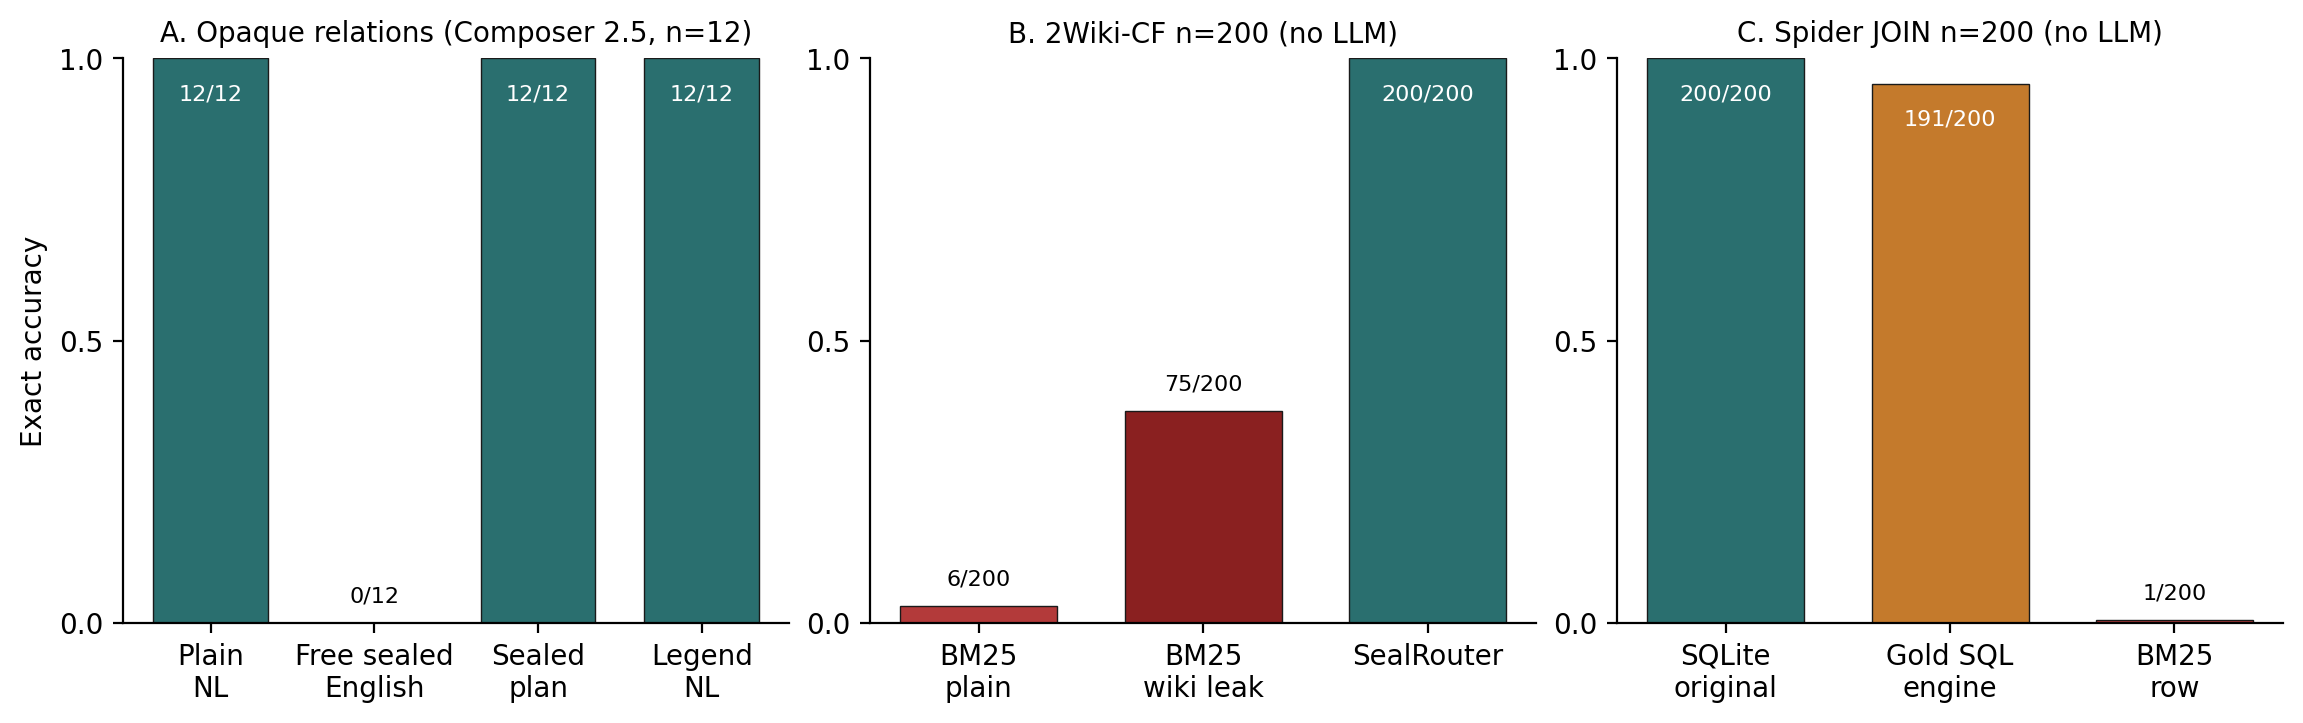
\includegraphics[width=\linewidth]{fig7_opaque_rel_n200.png}
\caption{Packaging and non-LLM controls.
Left: Composer $n{=}12$ (plain $12/12$, free sealed English $0/12$, plan $12/12$, legend $12/12$).
Middle: 2Wiki-CF lexical BM25 $6/200$ (not a 2Wiki eval), Wikipedia leak $75/200$, SealRouter $200/200$.
Right: Spider sqlite $n{=}200$ ($200/200$), gold-SQL $191/200$ (sealed names;
9 execution misses), lexical BM25 $1/200$~\citep{robertson2009bm25}.
Spider identifier-in-$q$ EQ $51/100$ is a different cell.}
\label{fig:packaging}
\end{figure}

\FloatBarrier
\section{MetaQA-style 2-hop templates}
\label{app:extended}
\label{app:metaqa32}

Not an evaluation on the official MetaQA 14K test split.
The $n{=}32$ freeze uses published 2-hop question wording on the public
movie graph; all 32 items are actor$\to$movie$\to$director vs.\ writer
(two same-type person tails; start in $q$; writer is the decoy).
Condition~A leaves \emph{directed}/\emph{starred} in $q$
(\texttt{OPAQUE\_REL\_QENG}).
Condition~B hashes question atoms except the bracketed start
(\texttt{OPAQUE\_REL\_QHASH}).
Those ARM lines name the condition, not two 2-hops.
Plaintext is $32/32$ for all three families.
Condition~A is OpenAI $32/32$, Composer $19/32$, Grok $15/32$.
Condition~B is OpenAI $25/32$, Composer $27/32$, Grok $14/32$
(plans $32/32$, $31/32$, $32/32$).
That cell is not \textsc{Movie-B}: Movie-B $n{=}100$ hashes the verbs
\emph{and} uses a two-hop ARM (locked two-path $3/100$; archived banner
$25/100$).
That $25/32$ is closer to that banner than to the locked topology
ARM, another prompt-surface gap
(Section~\ref{sec:movieb}).
Composer B $27/32$ exceeding A $19/32$ is that packing, not a two-path
opacity law.

\section{Sign-flip of the two-path opacity contrast}
\label{app:signflip}

Let $d_i=\mathbf{1}[\text{opaque correct}]-\mathbf{1}[\text{English correct}]$
and $c_i=d^{\mathrm{two}}_i-d^{\mathrm{unique}}_i$.
Of 32 \textsc{Wiki-H5} items, 24 have $c_i{=}{-1}$, one has $c_i{=}{-2}$,
7 have $c_i{=}0$; $T{=}{-}26$.
Unique-path opaque is $32/32$, so this item-level interaction contrast
copies the two-path McNemar ($25$ vs.\ $0$,
$p{=}2^{-24}{=}5.96{\times}10^{-8}$;~\citealp{mcnemar1947}).
The body reports those paired counts; $T$ is not a separate finding.
Opacity is not a randomized within-item treatment.

\end{document}
